\documentclass[a4paper,12pt,twoside]{memoir}

% Castellano
\usepackage[spanish,es-tabla]{babel}
\selectlanguage{spanish}
\usepackage[utf8]{inputenc}
\usepackage[T1]{fontenc}
\usepackage{lmodern} % Scalable font
\usepackage{microtype}
\usepackage{placeins}

% Pseudocódigo
\usepackage[longend, noline, ruled, linesnumbered, resetcount, spanish, spanishkw]{algorithm2e}


\usepackage{apalike}
\let\bibhang\relax
\usepackage{natbib}


\RequirePackage{booktabs}
\RequirePackage[table]{xcolor}
\RequirePackage{xtab}
\RequirePackage{multirow}

% Links
\PassOptionsToPackage{hyphens}{url}\usepackage[colorlinks]{hyperref}
\hypersetup{
	allcolors = {red}
}

% Ecuaciones
\usepackage{amsmath}

% Rutas de fichero / paquete
\newcommand{\ruta}[1]{{\sffamily #1}}

% Párrafos
\nonzeroparskip

% Huérfanas y viudas
\widowpenalty100000
\clubpenalty100000

% Imágenes

% Comando para insertar una imagen en un lugar concreto.
% Los parámetros son:
% 1 --> Ruta absoluta/relativa de la figura
% 2 --> Texto a pie de figura
% 3 --> Tamaño en tanto por uno relativo al ancho de página
\usepackage{graphicx}
\newcommand{\imagen}[3]{
	\begin{figure}[!h]
		\centering
		\includegraphics[width=#3\textwidth]{#1}
		\caption{#2}\label{fig:#1}
	\end{figure}
	\FloatBarrier
}

% Comando para insertar una imagen sin posición.
% Los parámetros son:
% 1 --> Ruta absoluta/relativa de la figura
% 2 --> Texto a pie de figura
% 3 --> Tamaño en tanto por uno relativo al ancho de página
\newcommand{\imagenflotante}[3]{
	\begin{figure}
		\centering
		\includegraphics[width=#3\textwidth]{#1}
		\caption{#2}\label{fig:#1}
	\end{figure}
}

% El comando \figura nos permite insertar figuras comodamente, y utilizando
% siempre el mismo formato. Los parametros son:
% 1 --> Porcentaje del ancho de página que ocupará la figura (de 0 a 1)
% 2 --> Fichero de la imagen
% 3 --> Texto a pie de imagen
% 4 --> Etiqueta (label) para referencias
% 5 --> Opciones que queramos pasarle al \includegraphics
% 6 --> Opciones de posicionamiento a pasarle a \begin{figure}
\newcommand{\figuraConPosicion}[6]{%
  \setlength{\anchoFloat}{#1\textwidth}%
  \addtolength{\anchoFloat}{-4\fboxsep}%
  \setlength{\anchoFigura}{\anchoFloat}%
  \begin{figure}[#6]
    \begin{center}%
      \Ovalbox{%
        \begin{minipage}{\anchoFloat}%
          \begin{center}%
            \includegraphics[width=\anchoFigura,#5]{#2}%
            \caption{#3}%
            \label{#4}%
          \end{center}%
        \end{minipage}
      }%
    \end{center}%
  \end{figure}%
}

%
% Comando para incluir imágenes en formato apaisado (sin marco).
\newcommand{\figuraApaisadaSinMarco}[5]{%
  \begin{figure}%
    \begin{center}%
    \includegraphics[angle=90,height=#1\textheight,#5]{#2}%
    \caption{#3}%
    \label{#4}%
    \end{center}%
  \end{figure}%
}
% Para las tablas
\newcommand{\otoprule}{\midrule [\heavyrulewidth]}
%
% Nuevo comando para tablas pequeñas (menos de una página).
\newcommand{\tablaSmall}[5]{%
 \begin{table}
  \begin{center}
   \rowcolors {2}{gray!35}{}
   \begin{tabular}{#2}
    \toprule
    #4
    \otoprule
    #5
    \bottomrule
   \end{tabular}
   \caption{#1}
   \label{tabla:#3}
  \end{center}
 \end{table}
}

%
% Nuevo comando para tablas pequeñas (menos de una página).
\newcommand{\tablaSmallSinColores}[5]{%
 \begin{table}[H]
  \begin{center}
   \begin{tabular}{#2}
    \toprule
    #4
    \otoprule
    #5
    \bottomrule
   \end{tabular}
   \caption{#1}
   \label{tabla:#3}
  \end{center}
 \end{table}
}

\newcommand{\tablaApaisadaSmall}[5]{%
\begin{landscape}
  \begin{table}
   \begin{center}
    \rowcolors {2}{gray!35}{}
    \begin{tabular}{#2}
     \toprule
     #4
     \otoprule
     #5
     \bottomrule
    \end{tabular}
    \caption{#1}
    \label{tabla:#3}
   \end{center}
  \end{table}
\end{landscape}
}

%
% Nuevo comando para tablas grandes con cabecera y filas alternas coloreadas en gris.
\newcommand{\tabla}[6]{%
  \begin{center}
    \tablefirsthead{
      \toprule
      #5
      \otoprule
    }
    \tablehead{
      \multicolumn{#3}{l}{\small\sl continúa desde la página anterior}\\
      \toprule
      #5
      \otoprule
    }
    \tabletail{
      \hline
      \multicolumn{#3}{r}{\small\sl continúa en la página siguiente}\\
    }
    \tablelasttail{
      \hline
    }
    \bottomcaption{#1}
    \rowcolors {2}{gray!35}{}
    \begin{xtabular}{#2}
      #6
      \bottomrule
    \end{xtabular}
    \label{tabla:#4}
  \end{center}
}

%
% Nuevo comando para tablas grandes con cabecera.
\newcommand{\tablaSinColores}[6]{%
  \begin{center}
    \tablefirsthead{
      \toprule
      #5
      \otoprule
    }
    \tablehead{
      \multicolumn{#3}{l}{\small\sl continúa desde la página anterior}\\
      \toprule
      #5
      \otoprule
    }
    \tabletail{
      \hline
      \multicolumn{#3}{r}{\small\sl continúa en la página siguiente}\\
    }
    \tablelasttail{
      \hline
    }
    \bottomcaption{#1}
    \begin{xtabular}{#2}
      #6
      \bottomrule
    \end{xtabular}
    \label{tabla:#4}
  \end{center}
}

%
% Nuevo comando para tablas grandes sin cabecera.
\newcommand{\tablaSinCabecera}[5]{%
  \begin{center}
    \tablefirsthead{
      \toprule
    }
    \tablehead{
      \multicolumn{#3}{l}{\small\sl continúa desde la página anterior}\\
      \hline
    }
    \tabletail{
      \hline
      \multicolumn{#3}{r}{\small\sl continúa en la página siguiente}\\
    }
    \tablelasttail{
      \hline
    }
    \bottomcaption{#1}
  \begin{xtabular}{#2}
    #5
   \bottomrule
  \end{xtabular}
  \label{tabla:#4}
  \end{center}
}



\definecolor{cgoLight}{HTML}{EEEEEE}
\definecolor{cgoExtralight}{HTML}{FFFFFF}

%
% Nuevo comando para tablas grandes sin cabecera.
\newcommand{\tablaSinCabeceraConBandas}[5]{%
  \begin{center}
    \tablefirsthead{
      \toprule
    }
    \tablehead{
      \multicolumn{#3}{l}{\small\sl continúa desde la página anterior}\\
      \hline
    }
    \tabletail{
      \hline
      \multicolumn{#3}{r}{\small\sl continúa en la página siguiente}\\
    }
    \tablelasttail{
      \hline
    }
    \bottomcaption{#1}
    \rowcolors[]{1}{cgoExtralight}{cgoLight}

  \begin{xtabular}{#2}
    #5
   \bottomrule
  \end{xtabular}
  \label{tabla:#4}
  \end{center}
}



\graphicspath{ {./img/} }

% Capítulos
\chapterstyle{bianchi}
\newcommand{\capitulo}[2]{
	\setcounter{chapter}{#1}
	\setcounter{section}{0}
	\setcounter{figure}{0}
	\setcounter{table}{0}
	\chapter*{#2}
	\addcontentsline{toc}{chapter}{#2}
	\markboth{#2}{#2}
}

% Apéndices
\renewcommand{\appendixname}{Apéndice}
\renewcommand*\cftappendixname{\appendixname}

\newcommand{\apendice}[1]{
	%\renewcommand{\thechapter}{A}
	\chapter{#1}
}

\renewcommand*\cftappendixname{\appendixname\ }

% Formato de portada
\makeatletter
\usepackage{xcolor}
\newcommand{\tutor}[1]{\def\@tutor{#1}}
\newcommand{\course}[1]{\def\@course{#1}}
\definecolor{cpardoBox}{HTML}{E6E6FF}
\def\maketitle{
  \null
  \thispagestyle{empty}
  % Cabecera ----------------
\noindent
\includegraphics[width=\textwidth]{cabecera}\vspace{1cm}%
  \vfill
  % Título proyecto y escudo informática ----------------
  \colorbox{cpardoBox}{%
    \begin{minipage}{.8\textwidth}
      \vspace{.5cm}\Large
      \begin{center}
      \textbf{TFG del Grado en Ingeniería Informática}\vspace{.6cm}\\
      \textbf{\LARGE\@title{}}
      \end{center}
      \vspace{.2cm}
    \end{minipage}

  }%
  \hfill\begin{minipage}{.20\textwidth}
    
\includegraphics[width=\textwidth]{escudoInfor}
  \end{minipage}
  \vfill
  % Datos de alumno, curso y tutores ------------------
  \begin{center}%
  {%
    \noindent\LARGE
    Presentado por \@author{}\\ 
    en Universidad de Burgos --- \@date{}\\
    Tutor: \@tutor{}\\
  }%
  \end{center}%
  \null
  \cleardoublepage
  }
\makeatother

\newcommand{\nombre}{Patricia Hernando Fernández} %%% cambio de comando

% Datos de portada
\title{Aplicación del Aprendizaje Semisupervisado en el descubrimiento de ataques a Sistemas de Recomendación}
\author{\nombre}
\tutor{Álvar Arnaiz González}
\date{\today}

\begin{document}

\maketitle


\newpage\null\thispagestyle{empty}\newpage


%%%%%%%%%%%%%%%%%%%%%%%%%%%%%%%%%%%%%%%%%%%%%%%%%%%%%%%%%%%%%%%%%%%%%%%%%%%%%%%%%%%%%%%%
\thispagestyle{empty}


\noindent
\includegraphics[width=\textwidth]{cabecera}\vspace{1cm}

\noindent D. Álvar Arnaiz González, profesor del departamento de Ingeniería Informática, área de Lenguajes y Sistemas Informáticos.

\noindent Expone:

\noindent Que la alumna D.ª \nombre, con DNI 71362977A, ha realizado el Trabajo final de Grado en Ingeniería Informática titulado <<Aplicación del Aprendizaje Semisupervisado en el descubrimiento de ataques a Sistemas de Recomendación>>.

\noindent Y que dicho trabajo ha sido realizado por el alumno bajo la dirección del que suscribe, en virtud de lo cual se autoriza su presentación y defensa.

\begin{center} %\large
En Burgos, {\large \today}
\end{center}

\vfill\vfill\vfill

% Author and supervisor
\begin{center}
\begin{minipage}{0.45\textwidth}
\begin{flushleft} %\large
Vº. Bº. del Tutor:\\[2cm]
D. Álvar Arnaiz González
\end{flushleft}
\end{minipage}
\hfill
\end{center}


\vfill

% para casos con solo un tutor comentar lo anterior
% y descomentar lo siguiente
%Vº. Bº. del Tutor:\\[2cm]
%D. nombre tutor


\newpage\null\thispagestyle{empty}\newpage




\frontmatter

% Abstract en castellano
\renewcommand*\abstractname{Resumen}
\begin{abstract}
En este primer apartado se hace una \textbf{breve} presentación del tema que se aborda en el proyecto.
\end{abstract}

\renewcommand*\abstractname{Descriptores}
\begin{abstract}
Palabras separadas por comas que identifiquen el contenido del proyecto Ej: servidor web, buscador de vuelos, android \ldots
\end{abstract}

\clearpage

% Abstract en inglés
\renewcommand*\abstractname{Abstract}
\begin{abstract}
A \textbf{brief} presentation of the topic addressed in the project.
\end{abstract}

\renewcommand*\abstractname{Keywords}
\begin{abstract}
keywords separated by commas.
\end{abstract}

\clearpage

% Indices
\tableofcontents

\clearpage

\listoffigures

\clearpage

\listoftables
\clearpage

\mainmatter
\capitulo{1}{Introducción}

A diferencia de unas décadas atrás, la sociedad actual está gobernada por los datos. La transición a la era de la información puede ser compleja para determinados colectivos y, consecuentemente, han surgido grupos que pretenden facilitar la experiencia de los usuarios, mientras que otros buscan aprovechar la falta de información general para lograr un beneficio.

Este trabajo de investigación pretende explorar cómo la minería de datos, en concreto el aprendizaje semisupervisado, puede aplicarse a la seguridad informática con el fin de lograr un entorno digital de confianza. Para ello, se han abierto dos ramas de investigación: la detección automática de ataques en sistemas de recomendación y la detección de \textit{phishing.}

Un sistema de recomendación es un algoritmo desarrollado con el fin de resumir información y facilitar la toma de decisiones. Son herramientas que pretenden realizar sugerencias de objetos que pueden resultar interesantes para un determinado perfil. Económicamente, este tipo de algoritmo es un claro objeto de interés, puesto que puede influir en la toma de decisiones de los compradores y hacer que se inclinen por un determinado producto (por ejemplo, el que tenga una mejor valoración). Los atacantes conocen esta situación y manipulan estas herramientas mediante el uso de perfiles falsos con el fin de beneficiar sus productos o perjudicar los de la competencia. Por ello, uno de los objetivos del proyecto es explorar cómo el aprendizaje semisupervisado puede ayudar a detectar los ataques a sistemas de recomendación, diferenciando entre perfiles genuinos e inyectados, además de comprobar la veracidad de los trabajos previos planteados por otros investigadores.

Por otro lado, se denomina \textit{phishing} a la técnica de ingeniería social en la que un atacante suplanta la identidad de una entidad de confianza con el fin de extraer datos o información personal de un determinado usuario. Este tipo de ataque es uno de los más comunes y peligrosos. Según el informe \textit{State of the Phish Report}, en el 2021, un 83\% de las empresas encuestadas sufrieron un ataque de estas características y el 54\% acabó con brechas de datos de clientes~\cite{phishingPorcentajeExito}. Por ello, se pretende crear un sistema de detección que permita distinguir enlaces falsos de auténticos mediante ténicas de aprendizaje semisupervisado.

\section{Estructura de la memoria}

El proyecto ha sido dividido en dos documentos independientes pero complementarios.

\subsection{Memoria}

Documento principal donde se pueden encontrar los siguientes apartados:

\begin{enumerate}
	\item \textbf{Introducción}: contextualización, estructura y recursos del proyecto.
	\item \textbf{Objetivos}: exposición de los pilares básicos del trabajo y las metas propuestas.
	\item \textbf{Conceptos teóricos}: descripción de los fundamentos principales necesarios para la correcta comprensión del documento.
	\item \textbf{Técnicas y herramientas}: enumeración de algunas de las técnicas y herramientas utilizadas durante el desarrollo del proyecto.
	\item \textbf{Aspectos relevantes del proyecto}: exposición y análisis de los experimentos realizados y las aproximaciones propuestas.
	\item \textbf{Trabajos relacionados}: comparación entre literatura existente desarrollada en el mismo ámbito que el trabajo presentado.
	\item \textbf{Conclusiones y líneas de trabajo futuras}: resumen de los aprendizajes obtenidos y proposición de ideas de mejora.
\end{enumerate}

\subsection{Anexos}

Documento orientado hacia el desarrollo del producto entregado, se divide en las siguientes secciones:

\begin{enumerate}
	\item \textbf{Plan de proyecto \textit{software}}: discusión acerca de la viabilidad temporal, económica y legal del producto presentado.
	\item \textbf{Especificación de requisitos}: análisis de las características que debe poseer el proyecto \textit{software} mediante el uso de catálogos, prototipos, diagramas y tablas.
	\item \textbf{Especificación de diseño}: descripción detallada de la estructura,
	el comportamiento y la interacción de la propuesta entregada.
	\item \textbf{Documentación técnica de programación}: recursos diseñados para disminuir la curva de aprendizaje y facilitar la inclusión de otros desarrolladores en el proyecto.
	\item \textbf{Documentación de usuario}: manuales necesarios para garantizar que el usuario final del producto pueda utilizar el \textit{software} con facilidad y reciba soporte adecuado.
\end{enumerate} 

\section{Enlaces adicionales}

Se facilita a continuación el acceso directo a los materiales del proyecto.

\begin{enumerate}
	\item Repositorio del proyecto:
	\url{https://github.com/phf1001/semisupervised-learning-in-cibersecurity}
	\item \textit{Web} desplegada en Heroku: \url{https://krini.herokuapp.com/index}
	\item Imágenes de Docker con la \textit{web} y su base de datos: \url{https://hub.docker.com/r/phf1001/krini/tags}
	\item \textit{Scripts} de despliegue en distintos sistemas operativos: \url{https://github.com/phf1001/semisupervised-learning-in-cibersecurity/tree/main/docker-deploy-kit}
\end{enumerate}
\capitulo{2}{Objetivos del proyecto}

Previo a la introducción de objetivos técnicos y de desarrollo, se facilita al lector el contexto en el que se desarrolla este proyecto de investigación con el fin de que se familiarice con el mismo.

\section{Contexto}
\label{contexto}

Es destacable que este proyecto se sostiene sobre tres pilares complementarios pero a su vez independientes.

\subsection{Aprendizaje semisupervisado}

Por un lado, en este trabajo se pretende ahondar en el campo de la minería de datos, más concretamente en el concepto de aprendizaje semisupervisado. Para ello, se van a implementar y validar diversos algoritmos de este tipo, en concreto el \textit{co-forest} (consultar aspectos teóricos en la sección~\ref{coforest-teoria} y la experimentación en la sección~\hyperref[coforest-exp]{5.1.1}), el \textit{tri-training} (secciones~\ref{tritraining-teoria} y~\hyperref[tritraining-exp]{5.1.2}) y el \textit{democratic-co learning} (secciones~\ref{democraticco-teoria} y~\hyperref[democraticco-exp]{5.1.3}).

Es reseñable que se pretende alcanzar un nivel de comprensión superior a la mera programación, realizando incluso pequeñas aportaciones a los algoritmos (basadas en la experimentación) en aquellos casos donde el pseudocódigo facilitado por los autores carezca de detalles de implementación.

\subsection{Ciberseguridad}

Implementar algoritmos es un ejercicio relevante, pero carece de sentido práctico si no pueden ser utilizados. Por ello, se pretende encontrar una aplicación a los mismos. Concretamente, se ha propuesto el modelado de un problema real relacionado con la ciberseguridad.

En un primer lugar se valoró estudiar la detección de ataques en sistemas de recomendación~\cite{zhou2021SemisupervisedRecommendationAttack}, pero se desestimó por su bajo desempeño. Finalmente, se ha escogido la detección de \textit{phishing}~\cite{featuresPhishing2018Gupta}. 

Es destacable que, previo a la selección de las ramas mencionadas anteriormente, se realizó una investigación en la literatura de la materia leyendo y comparando diversos tópicos como intrusión en redes, localización de \textit{markets} ilegales en la \textit{deep web}, detección de \textit{malware} o descubrimiento de dispositivos anómalos en redes IoT.

\subsection{Desarrollo y despliegue}

Por último, se pretende diseñar e implementar una herramienta que permita poner al servicio de la comunidad el conocimiento desarrollado. Se ha decidido crear un analizador de \textit{phishing} en formato página \textit{web}, permitiendo además la administración avanzada de modelos de \textit{machine learning} e instancias de aprendizaje. Además, se ha desplegado dicha herramienta utilizando Heroku\footnote{Disponible en \url{https://krini.herokuapp.com/index}.} y en local mediante Docker\footnote{\textit{Scripts} e instrucciones de despliegue disponibles en \url{https://github.com/phf1001/semisupervised-learning-in-cibersecurity/tree/main/docker-deploy-kit}.}.

\section{Objetivos}

Entendidos como las metas a alcanzar durante el desarrollo del proyecto, se pueden clasificar en dos secciones.

\subsection{Objetivos técnicos}
\label{Objetivos técnicos}

Se han propuesto los siguientes objetivos técnicos:

\begin{enumerate}
	\item \textbf{Implementar y evaluar distintos algoritmos de aprendizaje semisupervisado:} con rigor científico y procurando una codificación eficiente.
	\item \textbf{Experimentar con detalles de implementación no concretados:} para comprobar cómo determinadas decisiones pueden afectar el desempeño de un algoritmo.
	\item \textbf{Comparar contra implementaciones de terceros:} logrando unas condiciones de análisis justas.
	\item \textbf{Modelar un problema de ciberseguridad:} ofreciendo una solución práctica basada en el aprendizaje predictivo.
	\item \textbf{Establecer medidas de seguridad:} siendo consciente de que los métodos de extracción pueden ser vulnerables y mitigando el riesgo.
	\item \textbf{Evaluar la calidad de la solución aportada:} en términos de rendimiento.
	\item \textbf{Aprendizaje de nuevas tecnologías:} y familiarización con la programación \textit{web}.
	
\end{enumerate}

\subsection{Objetivos de desarrollo \textit{software}}
\label{Objetivos de desarrollo}

Se han propuesto los siguientes objetivos de desarrollo software:

\begin{enumerate}
	\item \textbf{Implementar de forma estándar los algoritmos:} siguiendo la interfaz de programación que establece Scikit-Learn (métodos \texttt{fit} y \texttt{predict}).
	\item \textbf{Adoptar metodologías ágiles de desarrollo} y familiarización con el flujo de trabajo de Scrum.
	\item \textbf{Documentar el producto desarrollado:} de forma concisa y que resuma, utilizando herramientas visuales y multimedia, la arquitectura planteada y su utilización.
	\item \textbf{Lograr un código de calidad:} desarrollando un producto que tenga una deuda técnica baja y una curva de aprendizaje asumible mediante el uso de herramientas como SonarCloud, DeepSource o GitGuardian.
	\item \textbf{Aplicar la integración y entrega continua:} de forma que se garantice el desarrollo de un producto mínimo viable que permita la detección temprana de errores y facilite la corrección al tutor.
	\item \textbf{Vincular fuentes de persistencia:} como bases de datos SQL.
	\item \textbf{Desplegar en plataformas:} logrando una familiarización con nuevas tecnologías en auge como Heroku y Docker.
	\item \textbf{Automatizar pruebas:} en distintas fases del ciclo de vida del producto mediante el uso de herramientas como TravisCI y Selenium.
	
\end{enumerate}
\capitulo{3}{Conceptos teóricos}

Se sintetizarán a continuación algunos de los conceptos teóricos más relevantes para la correcta comprensión del documento.

\section{Apendizaje automático}

Se denomina aprendizaje automático a aquella rama de la inteligencia artificial cuyo objetivo es desarrollar métodos que permitan que un algoritmo mejore su rendimiento mediante la experiencia y procesado de datos. Consecuentemente, los modelos entrenados realizarán predicciones cada vez más precisas como resultado del algoritmo implementado.

Se conoce como <<instancia>> (o entrada) a cada fila del \textit{dataset}. Estas están caracterizadas por atributos, que pueden ser numéricos (sus valores son números) o categóricos (sus valores son etiquetas, nombres, categorías, etc)~\cite{apuntesSisint}.

Dentro del aprendizaje automático se diferencian tres grandes grupos en función del tipo de entrada que sea consumida durante el entrenamiento~\cite{engelen2020surveyOnSemiSupervised}: el aprendizaje supervisado (datos etiquetados), el no supervisado (datos no etiquetados) y el semisupervisado (datos etiquetados y no etiquetados), siendo esta última categoría objeto de estudio en este proyecto de investigación. Se entiende por etiqueta como la representación de una determinada clase. 

El aprendizaje supervisado (vertiente predictiva) tiene como meta construir un clasificador (o regresor) que sea capaz de estimar el valor de salida para entradas nuevas (que no se hayan <<visto>> hasta el momento). Por otro lado, el aprendizaje no supervisado (vertiente descriptiva) trata de inferir la estructura interna de las entradas y agruparlas según similitudes (\textit{clustering}). Por último, el aprendizaje semisupervisado es la rama que pretende combinar estas dos vertientes complementándolas~\cite{engelen2020surveyOnSemiSupervised}. La aplicación más común de estos métodos es generar clasificadores efectivos cuando los datos disponibles son escasos, aunque no es la única.

Un clasificador generalmente cuenta con dos fases a lo largo de su ciclo de vida: la fase de entrenamiento y la fase de predicción. En la primera, el estimador trata de encontrar una hipótesis idéntica al concepto objetivo para todos los datos de entrenamiento, suponiendo que la mejor hipótesis para los datos no vistos es aquella que mejor se ajusta a los datos de entrenamiento~\cite{mitchell1997machine}. Es decir, trata de <<aprender>> sobre el conjunto de entrenamiento. Posteriormente, el clasificador está preparado para realizar predicciones en instancias nuevas.

El \textit{dataset} disponible inicialmente suele ser dividido en conjuntos más pequeños en función de su finalidad~\cite{apuntesSisint}. El conjunto de entrenamiento es aquel subconjunto de los datos utilizado para construir los modelos predictivos (generalmente, a mayor sea este conjunto mejor). Por otro lado, el conjunto de \textit{test} es un subconjunto menor no visto por el modelo (no utilizado durante el entrenamiento) utilizado para estimar el desempeño del modelo a posteriori.


\section{Aprendizaje semisupervisado}

Como se ha mencionado anteriormente, se denomina aprendizaje semisupervisado a aquel conjunto de algoritmos que utiliza datos etiquetados y no etiquetados para realizar tareas de aprendizaje. 

Cuando se habla de aprendizaje semisupervisado, hay ciertas suposiciones que se asumen, además de una condición: que la distribución marginal subyacente en el espacio de entradas $p(x)$ contenga información acerca de la posterior distribución $p(y|x)$~\cite{engelen2020surveyOnSemiSupervised}. Si no se cumple este requisito, no se puede segurar que las predicciones basadas en datos no etiquetados vayan a ser adecuadas, aunque en la mayoría de los casos de la vida real ocurre. Sin embargo, la forma en la que $p(x)$ y $p(y|x)$ interactúan no siempre es la misma, aunque se pueden esperar ciertos comportamientos plasmados en las <<suposiciones del aprendizaje semisupervisado>> (imagen~\ref{img:assumptions}). Entre ellas:

\begin{itemize}
	\item \textbf{\textit{Smoothness assumption}}: si dos muestras $x$ y $x'$ están cerca en el espacio de entrada, sus etiquetas $y$ y $y'$ deberían ser las mismas.
	
	\item \textbf{\textit{Low-density assumption}}: esta suposición propone que la frontera de decisión de un clasificador no debería cortar regiones con alta densidad de datos.
	
	\item \textbf{\textit{Mainfold assumption}}: postula que el espacio de entrada está compuesto por varios \textit{manifolds} (<<colectores>>) de dimensiones menores, y que todos los datos contenidos en un mismo \textit{manifold} tienen la misma etiqueta.
\end{itemize}


\begin{figure}[h]
	\caption[Suposiciones del aprendizaje semisupervisado]{\textit{Smoothness} y \textit{Low-density assumption} a la izquierda, \textit{Mainfold assumption} a la derecha. Extraída de \textit{A survey on semi-supervised learning}~\cite{engelen2020surveyOnSemiSupervised}.}
	\label{img:assumptions}
	\centering
	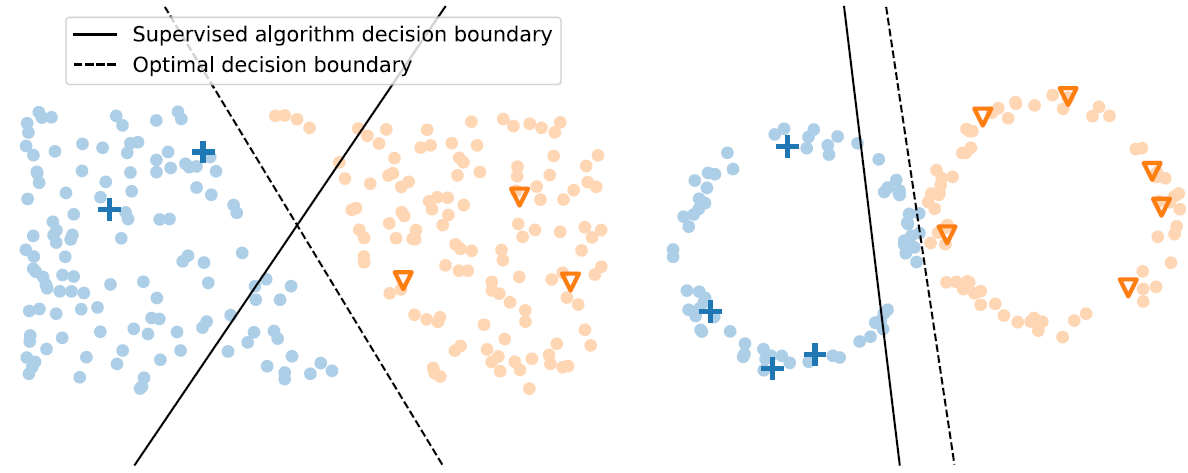
\includegraphics[width=\textwidth]{../img/memoria/3_assumptions}
\end{figure}


\subsection{Clasificación}

Inicialmente, se pueden diferenciar dos categorías~\cite{engelen2020surveyOnSemiSupervised}: los métodos inductivos, cuyo objetivo principal es construir un clasificador que genere predicciones para cualquier entrada y los métodos transductivos, cuyo poder de predicción está limitado a los objetos utilizados en la fase de entrenamiento.


\begin{figure}[h]
\caption[Taxonomía de métodos de aprendizaje semisupervisado]{Taxonomía de métodos de aprendizaje semisupervisados. Extraída de \textit{A survey on semi-supervised learning}~\cite{engelen2020surveyOnSemiSupervised}.}
\centering
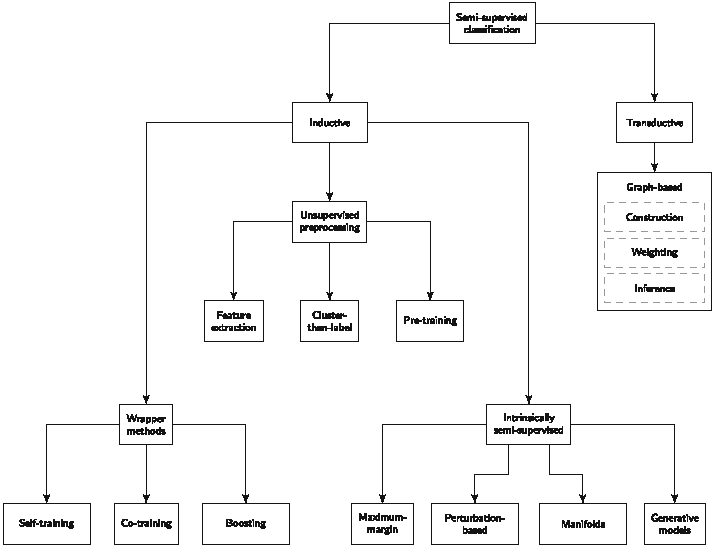
\includegraphics[width=\textwidth]{../img/memoria/3_hoos_taxonomy}
\end{figure}

Prescindiendo de los métodos transductivos por ser menos versátiles y útiles en nuestro propósito, los métodos inductivos se subdividen en tres grupos~\cite{engelen2020surveyOnSemiSupervised}: \textit{wrapper methods} (o métodos de envoltura), \textit{unsupervised preprocessing} y \textit{intrinsically semi-supervised}, siendo materia de estudio los métodos de envoltura. 


\subsection{Métodos de envoltura}

Estos modelos utilizan uno o más clasificadores que son entrenados iterativamente con los datos etiquetados de entrada, además de con datos pseudo-etiquetados. Se denomina pseudo-etiquetado a aquellos datos que inicialmente no estaban etiquetados, pero acabaron estándolo por iteraciones previas de los clasificadores.

Consecuentemente, el procedimiento consta de dos fases que se repiten en cada iteración: el entrenamiento y el pseudo-etiquetado. Durante el entrenamiento, los clasificadores se alimentan de datos etiquetados (o pseudo-etiquetados). En la fase de pseudo-etiquetado, se utilizan datos no etiquetados para que sean procesados por los clasificadores previamente entrenados. 

Dentro de esta categoría, se pueden diferenciar tres grandes grupos: \textit{self-training}, que utilizan únicamente un clasificador, \textit{co-training}~\cite{engelen2020surveyOnSemiSupervised}, que utilizan más de uno y los \textit{pseudo-labelled boosting methods}, que construyen clasificadores individuales que se alimentan de las predicciones más fiables. Se estudiará más en profundidad los métodos \textit{co-training}.

\subsubsection{Co-training}

En estos algoritmos, varios clasificadores son entrenados iterativamente utilizando datos etiquetados y añadiendo las predicciones (resultados) más confiables al conjunto para ser utilizadas en las siguientes iteraciones~\cite{engelen2020surveyOnSemiSupervised}. Para que los clasificadores sean capaces de generar información distinta, generalmente se divide el conjunto de entrada según alguna característica (no siendo estrictamente necesario). El \textit{co-forest}, algoritmo protagonista de este proyecto, pertenece a esta categoría.

Para que estos métodos tengan éxito, es importante que los clasificadores base no estén fuertemente correlacionados con sus predicciones, ya que entonces se limita el potencial para proporcionar información útil al resto~\cite{engelen2020surveyOnSemiSupervised}. Es decir, los estimadores han de ser diversos. Una de las formas de conseguir diversidad es mediante el uso de clasificadores inestables. Otra, obtener más de una vista del conjunto de datos inicial.


\section{\textit{Ensembles}}

Cuando se cuenta con un único estimador base a la hora de realizar una predicción, la etiqueta asignada es directamente la predicha por el clasificador. Sin embargo, en muchas ocasiones, puede resultar enriquecedor recurrir a lo estimado por más de un modelo~\cite{ensembles2006robi}. 

Se define \textit{ensemble} como un conjunto de modelos de \textit{machine learning} donde cada estimador base genera una predicción individual que se combina con el resto para generar una salida única~\cite{originalCoForest2007}.  Hay varios motivos por los que resulta favorecedor contar con un conjunto de clasificadores en lugar de con un único estimador base~\cite{ensembles2006robi}:

\begin{itemize}
	\item \textbf{Motivos estadísticos:} en muchas ocasiones se obtienen buenos resultados en los datos de entrenamiento, pero un error de generalización alto. También se puede dar el caso en el que un conjunto de clasificadores con resultados similares en el conjunto de prueba actúe de manera distinta en la aplicación real (el conjunto de \textit{test} no es lo suficientemente representativo). En estos casos, el hecho de contar con un conjunto de clasificadores reduce considerablemente las probabilidades de predecir mal una etiqueta. Una analogía en la vida real sería cuando se pide opinión médica a un conjunto de doctores (y no a uno solo) para obtener un diagnóstico no sesgado por las experiencias previas de un sólo médico.
	
	\item \textbf{Gran cantidad de datos:} cuando la cantidad de información es demasiada, puede no ser manejada correctamente por un único clasificador. Por ello, es mejor particionarla en distintos conjuntos de entrenamiento y prueba, y alimentar cada modelo con una partición.
	
	\item \textbf{Escasa cantidad de datos:} si los datos no son suficientes, puede ocurrir que un clasificador no sea capaz de aprender su estructura interna. Por ello, es recomendable realizar un muestreo de los datos (con reemplazo) y entrenar varios modelos distintos con ellos. De esta manera, los errores disminuyen.
	
	\item \textbf{Divide y vencerás:} cuando un problema es demasiado complicado de resolver utilizando un único clasificador, utilizar un conjunto de ellos puede ser efectivo.
\end{itemize}


\subsection{Diversidad y clasificación}

En la realidad, los datos contienen ruido, \textit{outliers}, distribuciones que se solapan, etc. Por ello, es muy complicado obtener un clasificador con un desempeño perfecto~\cite{ensembles2006robi}. Los \textit{ensembles} reducen el error cometido por cada estimador base debido a que combinan las salidas de los mismos. Puede parecer <<negativo>> que los clasificadores individuales difieran. Sin embargo, la realidad es que cuanto más único sea cada estimador utilizado y más distintas sean sus \textit{decision boundaries} (frontera que divide la superficie del problema en partes), mejor.

Esta diversidad se puede obtener de distintas formas, por ejemplo, utilizando distintos conjuntos de entrenamiento y \textit{test} en los estimadores base (utilizando técnicas de \textit{bootstrapping}, por ejemplo). Otra opción muy destacable es utilizando clasificadores <<inestables>> (aquellos que sean muy distintos con pequeños cambios en el conjunto de entrenamiento), como por ejemplo los árboles.

A la hora de crear un \textit{ensemble}, hay dos preguntas clave que realizarse: ¿cómo se van a generar los clasificadores base? ¿cómo van a diferenciarse los unos de los otros?~\cite{ensembles2006robi}.

Para lograr un mayor nivel de diversidad, se pueden utilizar procedimientos de muestreo o selección de parámetros. En función de ellos y de cómo se realice el entrenamiento (consultar imagen~\ref{img:bagging}), los \textit{ensembles} pueden ser de distintos tipos.
	
\subsubsection{\textit{Bagging (Random Forest)}}

El \textit{bagging} es uno de los modelos más antiguos y populares~\cite{ensembles2006robi}. Se compone de un conjunto de estimadores base entrenados en paralelo. Por lo tanto, el resultado es el promedio (o más popular) de las salidas de los modelos simples. Para entrenar cada estimador base se utiliza \textit{bootstrapping}~\cite{engelen2018thesis}, que es una técnica de muestreo que genera un subconjunto de datos seleccionando aleatoriamente muestras de un conjunto mayor permitiendo la repetición. Es decir, los clasificadores son entrenados con un subconjunto aleatorio del total de los datos etiquetados como se ilustra en la figura~\ref{img:bagging}. Esta técnica puede ser utilizada con o sin reemplazo, entendiendo que el muestreo con reemplazo se produce cuando cada una de las unidades maestrales seleccionada es devuelta a la población total antes de extraer la siguiente (puede repetirse).

El \textit{bagging} es muy útil cuando se dispone poca cantidad de datos, y la cantidad de muestras que contiene cada conjunto de entrenamiento es de entre el $75\% - 100\%$ del total del \textit{dataset}~\cite{ensembles2006robi}. Al utilizar \textit{bootstrapping}, los conjuntos de \textit{test} se suelen solapar, además de poder contener muestras repetidas (reemplazo). Por ello, es recomendable utilizar clasificadores base inestables, como por ejemplo los árboles.

Cuando todos los estimadores base son árboles, se habla de \textbf{\textit{random forest}}, uno de los métodos de \textit{bagging} más populares que obtiene resultados certeros debido a la aleatoriedad introducida~\cite{originalCoForest2007}. Cuando el \textit{ensemble} devuelve una etiqueta, es el resultado de una votación realizada por todos los árboles del conjunto. Además de utilizar \textit{bootstrapping}, en el entrenamiento individual de cada árbol, únicamente se <<ven>> algunos atributos (no el total) para introducir mayor aleatoriedad. Es decir, en cada nodo del árbol solo se tienen en cuenta ciertas características seleccionadas aleatoriamente.

\begin{figure}[h]
	\caption[Entrenamiento \textit{bagging} y \textit{boosting}]{Diferencias entre el entrenamiento en \textit{bagging} (izquierda) y \textit{boosting} (derecha).}
	\label{img:bagging}
	\centering
	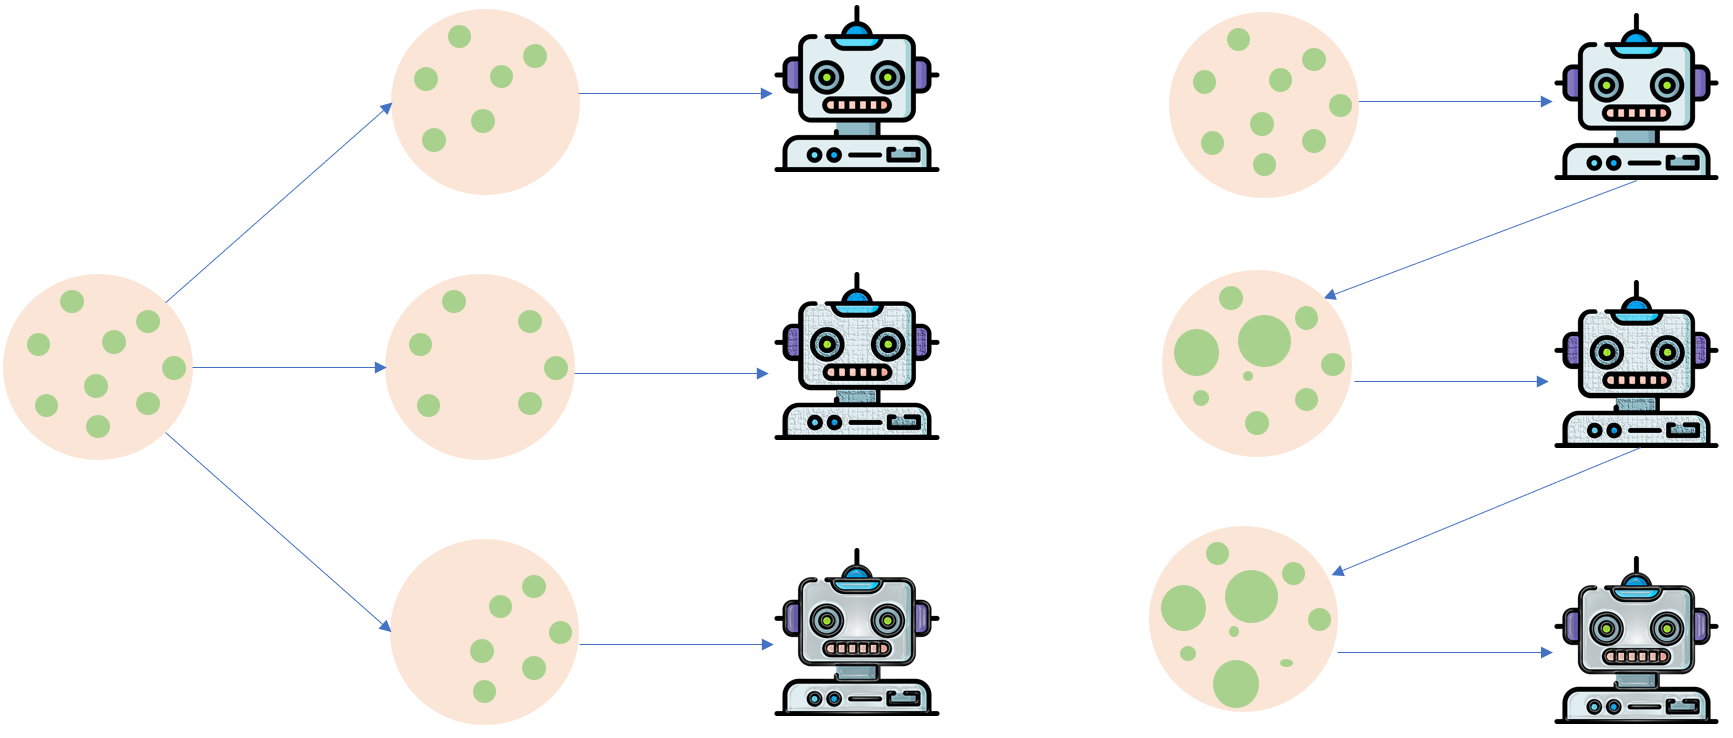
\includegraphics[width=\textwidth]{../img/memoria/3_bagging_boosting}
\end{figure}
	
\subsubsection{\textit{Boosting}}

Si el anterior modelo utiliza los clasificadores base <<en paralelo>>, este lo haría <<en serie>>~\cite{engelen2018thesis}. Es decir, hay un orden secuencial: los estimadores dependen del resultado anterior y tratan de compensar el error que se haya podido cometer (los \textit{weak learners} se convierten en \textit{strong learners}~\cite{ensembles2006robi}).

El entrenamiento se focaliza, por lo tanto, en torno a las instancias que hayan fallado los clasificadores previos. Esto se consigue dando más peso a aquellas muestras mal clasificadas. Por ejemplo, en problemas de regresión, las predicciones con un mayor error cuadrático medio tendrán más peso para el siguiente modelo. En clasificación, los estimadores se entrenan con aquellas muestras en las que los otros elementos del \textit{ensemble} difieran.

\subsection{Combinación de los clasificadores}

Suponiendo que sólo se dispone de las etiquetas asignadas por los clasificadores base como salida, hay diversos modos de <<fusionar>> los \textit{outputs} en uno único~\cite{ensembles2006robi}.

En el caso de que todos los estimadores base sean <<iguales>>, es frecuente utilizar \textit{majority voting} (<<votación de la mayoría>>). Cuenta con tres versiones: la votación unánime (todos los clasificadores coinciden), la mayoría simple (coincidencia de más del $50\%$ de los votos) y la votación por mayoría (la etiqueta que más votos haya recibido, representado en la ilustración~\ref{img:voting}).

Sin embargo, si se sabe que algunos clasificadores son mejores que otros, se puede aplicar \textit{weighted majority voting}, donde las etiquetas predichas por los estimadores con mejor rendimiento tienen más peso que el resto (se asigna una proporción).

\begin{figure}[h]
	\caption[Combinación mediante votación en \textit{ensembles}]{Representación de la combinación mediante votación.}
	\label{img:voting}
	\centering
	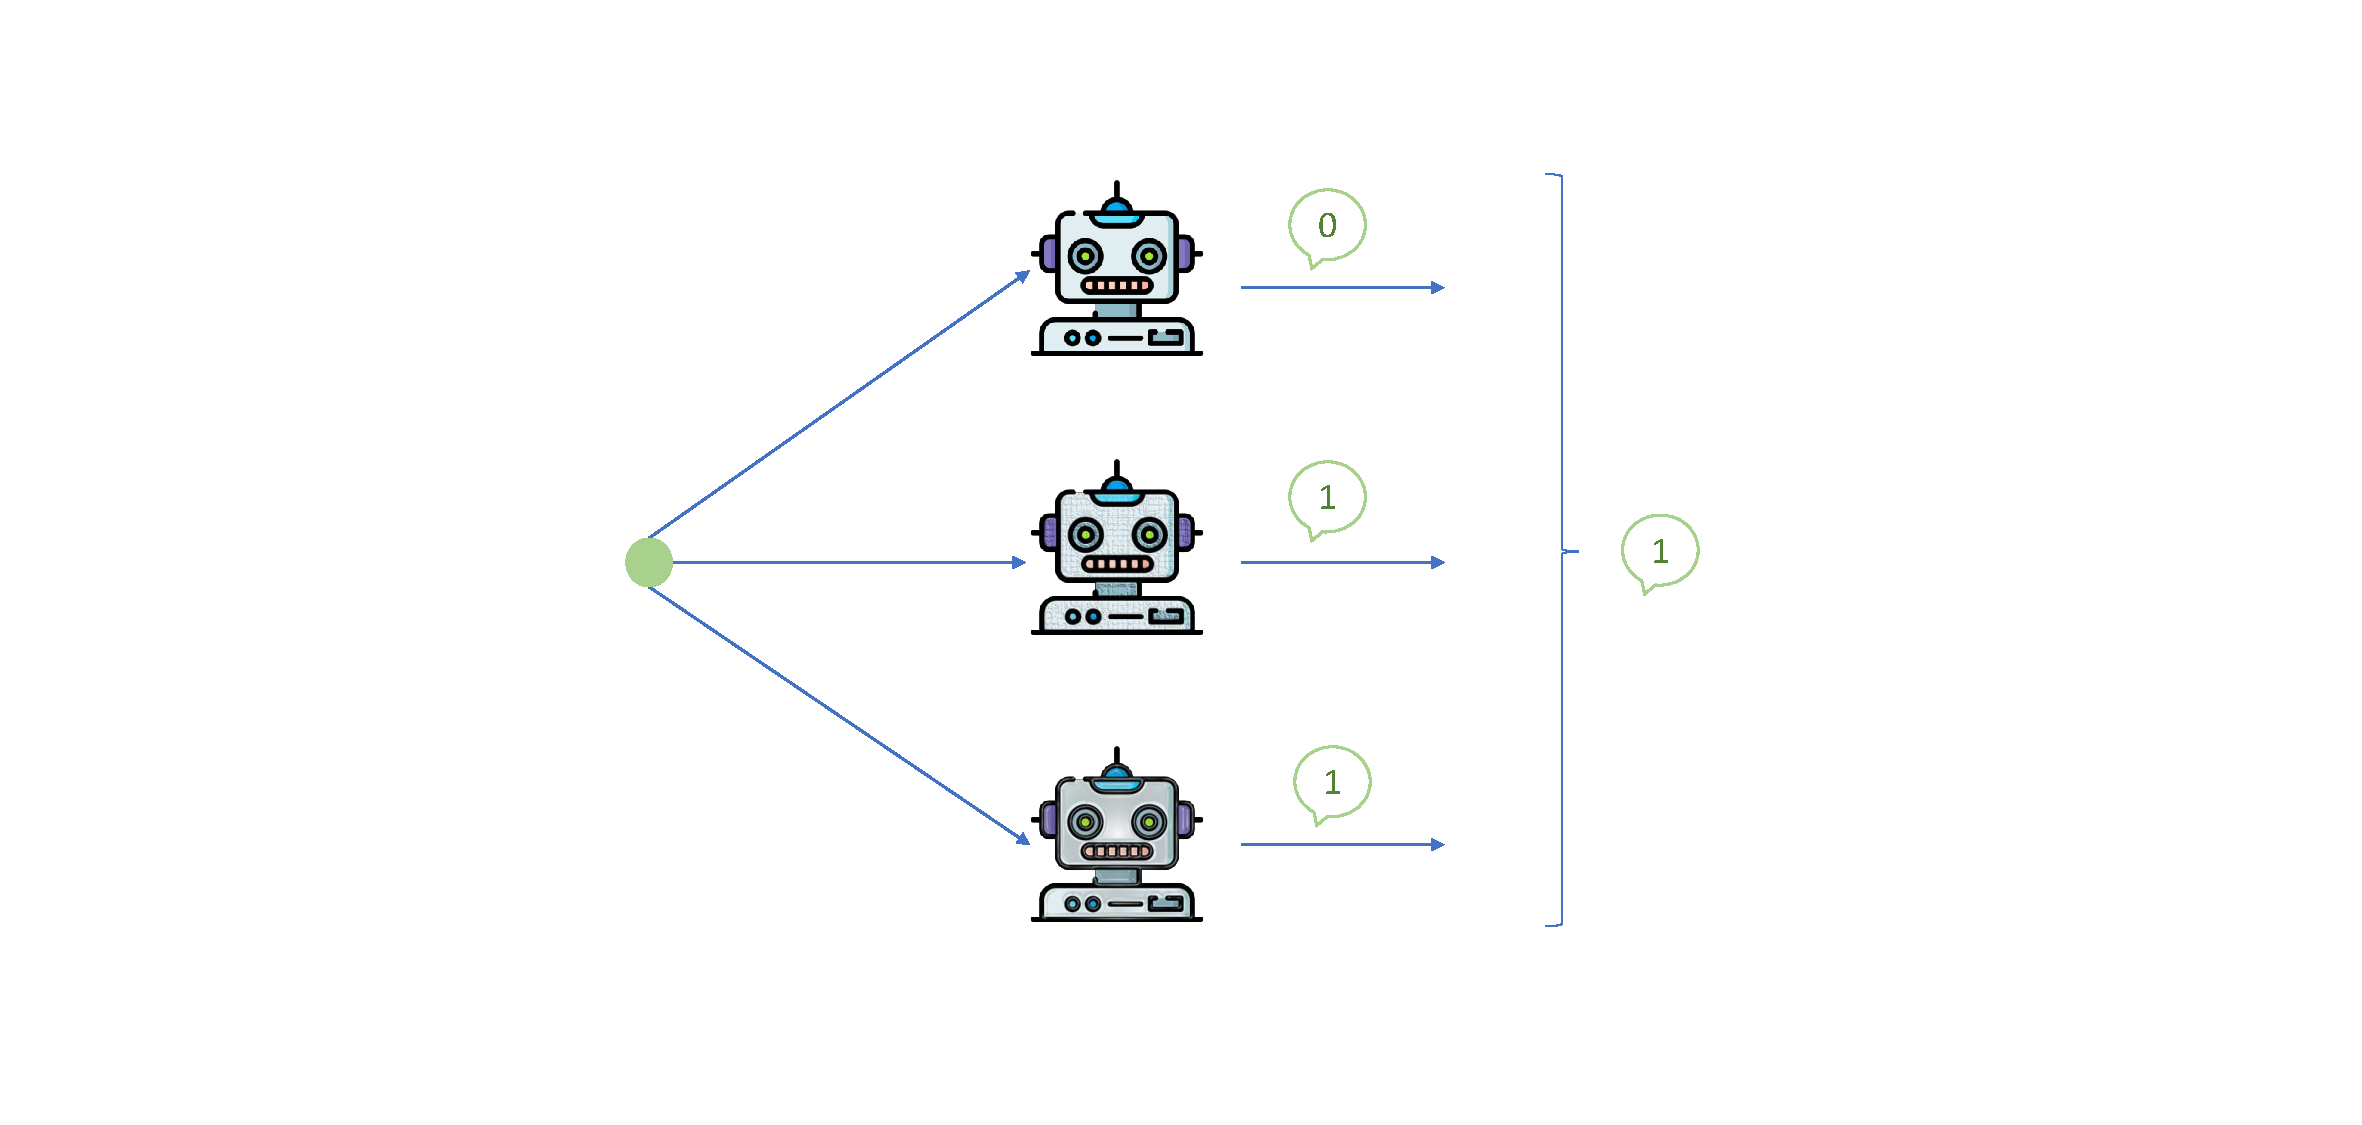
\includegraphics[scale=0.35]{../img/memoria/3_voting}
\end{figure}



\section{Métricas de evaluación}

En este trabajo de investigación se van a realizar continuamente comparaciones entre modelos de clasificación. Para ello, es necesario definir unas métricas. Estas se basan en conceptos que se exponen a continuación~\cite{apuntesSisint}:

\begin{itemize}
	\item \textbf{Verdadero positivo o \textit{True positive}}: se obtiene cuando un clasificador acierta en su predicción y esta es la clase de interés. Generalmente es la clase <<positiva>> y, en el caso de la aplicación en la detección de ataques a sistemas de recomendación, la <<minoritaria>>.
	\item \textbf{Verdadero negativo o \textit{True negative}}: resultado obtenido cuando un clasificador acierta en su predicción y esta no es la clase de interés.
	\item \textbf{Falso positivo o \textit{False positive}}: se obtiene cuando un clasificador falla en su predicción y predice que es la clase de interés, cuando en realidad no lo es.
	\item \textbf{Falso negativo o \textit{False negative}}: resultado obtenido cuando un clasificador falla en su predicción y afirma que una muestra no pertenece a la clase de interés, cuando en realidad sí pertenece.
	
	\item \textbf{Total}: la suma de los cuatro puntos anteriores equivale al total de predicciones ($T = TP + TN + FP + FN$).
	\item \textbf{\textit{Class imbalance problem}}: es un problema que se genera cuando hay muy pocas instancias positivas en el conjunto de datos en comparación con las negativas (es decir, cuando hay un desequilibro evidente entre ambas clases). Generalmente, causa que la \textit{accuracy} (consultar ecuación~\ref{eqn:accuracy}) sea muy elevada, pero no se detecten instancias de la clase positiva, generando modelos inservibles.
\end{itemize}

Dadas las definiciones anteriores, se facilitan las siguientes métricas utilizadas~\cite{apuntesSisint}:

\begin{itemize}
	\item \textbf{\textit{Accuracy}, exactitud o porcentaje de acierto}: mide la tasa de aciertos de un determinado clasificador. A lo largo del proyecto, también es llamada <<\textit{score}>>.
	
	\begin{equation}\label{eqn:accuracy} Accuracy = \frac{|Aciertos|}{|Total|} = \frac{TP + TN}{TP + TN + FP + FN} \end{equation}
	
	\item \textbf{\textit{Error rate}, o porcentaje de error}: mide la tasa de error del clasificador.
	
	\begin{equation}\label{eqn:error} Error Rate = \frac{|Fallos|}{|Total|} = \frac{FP + FN}{TP + TN + FP + FN} = 1 - Accuracy \end{equation}
	
	\item \textbf{Precisión}: mide cuántas predicciones son verdaderamente positivas entre todas las seleccionadas como tal.
	
	\begin{equation}\label{eqn:precision} Precision = \frac{TP}{TP + FP}\end{equation} 
	
	\item \textbf{\textit{Recall} o \textit{sensitivity}}: determina la capacidad del clasificador para detectar clases positivas. En otras palabras, determina el porcentaje de positivos detectados sobre el total de positivos reales.
	
	\begin{equation}\label{eqn:recall} Recall = \frac{TP}{TP + FN}\end{equation}
	
	\item \textbf{\textit{Specificity}}: determina cuántos elementos negativos son detectados.
	\begin{equation}\label{eqn:specificity} Specificity = \frac{TN}{TN + FP}\end{equation}
	
	\item \textbf{\textit{False positives ratio}}: determina cuántos negativos son clasificados como positivos sobre el total de negativos.
	
	\begin{equation}\label{eqn:FPR} FPR = \frac{FP}{FP + TN}\end{equation}
	
	\item \textbf{\textit{F-Measure}}: medida que combina la \textit{precision} y el \textit{recall}. Es de interés puesto que la meta general suele ser maximizar estas dos medidas.
	
	\begin{equation}\label{eqn:f-measure} \textrm{F-Measure} = 2 \times \frac{precision \times recall}{precision + recall} = \frac{ 2 \times TP}{2 \times TP + FP + FN} \end{equation}
	
	\item \textbf{\textit{AUC}}: área bajo la curva (\textit{area under curve}) \textit{ROC} (\textit{operating characteristic curve}). La curva \textit{ROC} es una representación gráfica del \textit{recall} frente a la \textit{specificity}. Cuando una curva es perfecta, su área es $1$.
	
	
\end{itemize}


\section{\textit{Co-forest}}

\subsection{Descripción}

El denominado \textit{co-forest}~\cite{originalCoForest2007} es un método de clasificación para aprendizaje semisupervisado (más concretamente, de envoltura) que permite construir un \textit{ensemble} de árboles de decisión (clasificación). Este método está basado en el \textit{random forest} y se podría considerar su <<versión semisupervisada>>. 

Que sea un algoritmo semisupervisado implica que, durante la fase de entrenamiento, además de utilizar el conjunto de datos etiquetados ($L$), se utilicen también aquellas pseudo-etiquetas de las predicciones con mejor confianza del conjunto de datos no etiquetados ($U$).

El proceso de entrenamiento se realiza iterativamente~\cite{engelen2018thesis}, y en cada una de estas repeticiones, se examina cada árbol y se entrena individualmente con un subconjunto de $L$ ($L_{i}$) y con un subconjunto de $U$ ($L'_{i,t}$) formado por aquellas pseudo-etiquetas que, además de pertenecer a la submuestra (aleatoria), posean un nivel de confianza superior a un umbral definido por el usuario ($\theta$). Quienes estiman esta confianza de predicción para las muestras seleccionadas son el conjunto de todos los árboles que forman el \textit{ensemble} menos el árbol que está siendo entrenado individualmente (de ahora en adelante \textit{concomitant ensemble} o conjunto concomitante).

El criterio de parada de la fase de entrenamiento del \textit{co-forest} es el \textit{out-of-bag error}~\cite{zhou2021SemisupervisedRecommendationAttack} (de ahora en adelante, OOBE). Se define OOBE como el error que comete el conjunto concomitante de un árbol para el total de los datos etiquetados. Es decir, el número de árboles que aciertan la etiqueta entre el número de árboles que votan teniendo en cuenta que, para calcular el OOBE del total de los datos etiquetados, sólo votan aquellos árboles que no hayan utilizado la muestra concreta de $L$ para su entrenamiento.


\subsection{Algoritmo}


\subsubsection{Variables utilizadas}

Para facilitar la comprensión del pseudocódigo, se definen a continuación algunas de las variables utilizadas:
\begin{itemize}
	\item $n$: número total de árboles del ensemble.
	\item $h_{i}$: árbol i-ésimo del conjunto.
	\item $H_{i}$: \textit{concomitant ensemble} o conjunto concomitante del árbol i-ésimo (todos los árboles del \textit{co-forest} menos él).
	\item $x_j$: muestra j-ésima (generalmente sin etiqueta).
	\item $H_i(x_j)$: etiqueta asignada por $H_i$ a la muestra j-ésima.
	\item $w_{i,t,j}$: confianza de predicción (individual) calculada para una muestra $x_j$ por $H_{i}$ en la iteración $t$. Se define confianza como el grado de acuerdo que existe en una votación. 
	\item $W$: sumatorio de las confianzas de predicción individuales de un conjunto $W = \sum w_{i,t,j}$.
	\item $L$: conjunto de datos etiquetados utilizados durante el entrenamiento.
	\item $L_{i}$: subconjunto obtenido tras aplicar \textit{bootstrapping} a $L$ que se utiliza para entrenar el árbol $h_{i}$.
	\item $U$: conjunto de datos no etiquetados utilizados durante el entrenamiento.
	\item $U'_{i,t}$: subconjunto aleatorio de U cuya $W$ es menor que $W_max$ (consultar ecuación~\ref{eqn:Wmax}).
	\item $L'_{i,t}$: subconjunto formado por aquellas muestras de $U'_{i,t}$ cuya confianza de predicción es superior a $\theta$.
	\item $\theta$: nivel de confianza mínimo que tiene que tener el clasificador al predecir la etiqueta de una muestra de $U$ para ser utilizada durante el entrenamiento de un árbol.
	\item $\hat{e}_{i,t}$: OOBE cometido por $H_{i}$ en $L$ en el instante de tiempo $t$.
\end{itemize} 

\subsubsection{Pseudocódigo}

Se facilita a continuación la versión del \textit{co-forest} de la tesis de Engelen~\cite{engelen2018thesis}, basada en la original~\cite{originalCoForest2007}, pero introduciendo los cambios observables en la sección <<Discusión de los parámetros del algoritmo>>.

\begin{algorithm}
	\KwIn{Conjunto de datos etiquetados $L \lbrace\left(x_i, y_i\right)\rbrace_{i=1}^l$, conjunto de datos no etiquetados $U \lbrace x_i \rbrace_{i=l+1}^{k}$, número de árboles $n$ y umbral de confianza $\theta$}
	\KwOut{\textit{Ensemble} de árboles entrenado $H$.}
	\BlankLine
	\For{$i$ = 0, ..., $n-1$}{
		$L_{i} \leftarrow$ Bootstrap($L$)\\
		$h_i$ = EntrenarArbol($L_{i}$)\\
		$\hat{e}_{i,t} \leftarrow 0.5$\\
		$W_{i,0} \leftarrow min(\frac{1}{10}|$U$|, 100)$\\
	}

	$t \leftarrow 0$\\
	\While(){Algún árbol reciba pseudo-etiquetas}{
	$t \leftarrow t + 1$\\
	
	\For{$i$ = 0, ..., $n-1$}{
		$\hat{e}_{i,t} \leftarrow$ OOBE($H_i, L$)\\
		$L'_{i,t} \leftarrow \emptyset$\\
		
		\If{$\hat{e}_{i,t} < \hat{e}_{i,t-1}$}{
			$W_{max} = \hat{e}_{i,t-1}W_{i,t-1}/\hat{e}_{i, t}$\\
			$U'_{i,t} \leftarrow$ Submuestrear($U, H_i, W_{max}$)\\
			$W_{i,t} \leftarrow 0$
			
			\ForEach{$x_j \in U'_{i,t}$}{
				
				\If{Confianza($H_i, x_j$) > $\theta$}{
					$L'_{i,t} \leftarrow L'_{i,t} \cup {x_j, H_i(x_j)}$\\
					$W_{i,t} \leftarrow W_{i,t} + Confianza(H_i, x_j)$
				}
			}
		}
	}
	\For{$i$ = 0, ..., $n-1$}{
		\If{$(e_{i,t} * W_{i,t} < e_{i, t-1} * W_{i, t-1})$}{
			$h_i$ = EntrenarArbol($L_{i} \cup L'_{i,t}$)\\
		}
	}
}
	\Return{$H$}

	\caption{\textit{Co-Forest}}\label{alg:co-forest}
	\end{algorithm}

\subsubsection{Fases}

En primer lugar, se ha de construir un \textit{random forest} de $n$ árboles. Para introducir aleatoriedad, cada uno de esos árboles es entrenado utilizando un subconjunto aleatorio de $L$. Es decir, un subconjunto obtenido tras aplicar \textit{bootstrap} a $L$.

Otro parámetro a tener en cuenta es el número de atributos a considerar en cada árbol de decisión. Por defecto, se ha establecido este valor al $log_{2}$ del total (heurística de Breiman~\cite{engelen2018thesis}). Sin embargo, también podría ser el la raíz cuadrada del total o el total, entre otros.

La segunda fase es entrenar el \textit{random forest} de manera semisupervisada e iterativa hasta que se cumpla el criterio de parada (como se ha mencionado anteriormente, basado en el OOBE). Para ello, se calcula el OOBE de un árbol para una iteración. Si es superior al anterior, se considera que el rendimiento ha empeorado para ese árbol. El algoritmo finaliza cuando todos los árboles empeoran su rendimiento en una determinada iteración.

Por el contrario, en caso de que se haya mejorado, se toma una submuestra de $U$ para pseudo-etiquetar (evidentemente, distinta para cada árbol). Posteriormente se examina cada una de las muestras que forman $U'_{i, t}$, y en caso de que el nivel de confianza supere el umbral, se selecciona esa muestra para el entrenamiento (pasa a formar parte de $L'_{i, t}$).

El último paso sería reentrenar los árboles que hayan cambiado con su propio conjunto inicial de datos etiquetados unido a las pseudo-etiquetas generadas en la correspondiente iteración ($L_{i}\cup L'_{i,t}$). Es decir, en cada iteración se considera $U$ al completo para poder generar la muestra con la que se pseudo-etiquete, y las anteriores pseudo-etiquetas para un árbol en concreto son descartadas~\cite{engelen2018thesis}.


\subsection{Tratamiento del ruido y teoría de errores}

Como se señala en el \textit{paper} de Zhou y Duan~\cite{zhou2021SemisupervisedRecommendationAttack}, de acuerdo con el trabajo de Angluin y Laird~\cite{noisyExamplesCoforest1988Dana}, si el tamaño de los datos utilizados en el entrenamiento ($m$), la tasa de ruido ($\eta$), el error de la hipótesis en el peor caso ($\epsilon$) y una constante ($c$) cumplen la relación de la ecuación~\ref{eqn:rel_convergencia_hipotesis}, entonces la hipótesis aprendida por el árbol $h_{i}$ (que minimiza el desacuerdo en un conjunto de muestras de entrenamiento con ruido) converge a la hipótesis verdadera.

\begin{equation}\label{eqn:rel_convergencia_hipotesis} m = \frac{c}{\epsilon^{2}(1-2\eta)^{2}} \end{equation} 

De acuerdo con~\cite{zhou2021SemisupervisedRecommendationAttack}, se puede obtener la función de utilidad mostrada en la ecuación~\ref{eqn:operar_rel_convergencia} operando en la expresión~\ref{eqn:rel_convergencia_hipotesis}.

\begin{equation}\label{eqn:operar_rel_convergencia} f = \frac{c}{\epsilon^{2}} = m(1-2\eta)^{2} \end{equation} 

Como se ha mostrado en el pseudocódigo, en la iteración i-ésima un determinado árbol se entrena con sus datos etiquetados $L_{i}$ y un conjunto de pseudo-etiquetas $L'_{i,t}$. Si se considera que el OOBE cometido en $L$ por $H_{i}$ es $\hat{e}_{i,t}$, entonces se puede estimar que el número de pseudo-etiquetas erróneas en $L'_{i,t}$ equivale a $\hat{e}_{i,t} \times W_{i,t}$ (se recuerda al lector que $W_{i,t}$ es el sumatorio de la confianza de predicción (grado de acuerdo) de $H_{i}$ en cada muestra de $L'_{i,t}$). Por lo tanto, la tasa de ruido que se encuentra en $L_{i} \cup L'_{i,t}$ es la estimada por la ecuación~\ref{eqn:ruido_it}, donde $W_0$ y $\eta_0$ son los parámetros correspondientes a $L$. 

\begin{equation}\label{eqn:ruido_it} \eta = \frac{\eta_{0}W_{0} + \hat{e}_{i,t}W_{i,t}}{W_{0} + W_{i,t}} \end{equation} 

De acuerdo con la ecuación~\ref{eqn:operar_rel_convergencia}, la función de utilidad $f$ es inversamente proporcional a $\epsilon^2$. Por lo tanto, si se quiere reducir el error cometido, se debe aumentar la utilidad de cada árbol en cada iteración~\cite{zhou2021SemisupervisedRecommendationAttack}. Consecuentemente, se debe cumplir la ecuación~\ref{eqn:relacion_e_W}. 

\begin{equation}\label{eqn:relacion_e_W} \frac{\hat{e}_{i,t}}{\widehat{e}_{i, t-1}} < \frac{W_{i,t-1}}{W_{i,t}} < 1 \end{equation} 


\subsubsection{Discusión acerca de los parámetros del algoritmo}

Intuitivamente se puede deducir la ecuación~\ref{eqn:relacion_e_W}, ya que el error debe disminuir y la confianza de predicción aumentar con cada iteración. Sin embargo, aunque esto se cumpla, puede ser que se deje de cumplir que $\hat{e}_{i,t}W_{i,t} < \hat{e}_{i,t-1}W_{i,t-1}$, ya que puede ocurrir que $ W_{i,t} >>> W_{i,t-1}$. Por este motivo y para cumplir con lo expuesto en la ecuación~\ref{eqn:relacion_e_W}, se limita $W_{max}$ como se muestra en la ecuación~\ref{eqn:Wmax} al realizar el muestreo de $U$ en el algoritmo.

\begin{equation}\label{eqn:Wmax} W_{max} = \frac{\hat{e}_{i,t-1}W_{i,t-1}}{\hat{e}_{i, t}} > W_{i,t} \end{equation}


\label{parag:Wmax_inicial} El algoritmo original propuesto por~\cite{originalCoForest2007} y el utilizado en~\cite{zhou2021SemisupervisedRecommendationAttack} dejan, sin embargo, una cuestión pendiente. Como se puede observar en la ecuación~\ref{eqn:Wmax}, $W_{max}$ requiere para calcularse tanto el OOBE como la $W$ obtenida en la iteración anterior, y ambos autores inician $W$ a 0. Esto implica que en la primera iteración $W_{max} = 0$ y, por lo tanto, evita que se realice un muestreo de $U$ para pseudo-etiquetar (pararía el algoritmo). En su tesis, Engelen~\cite{engelen2018thesis} propone solucionar este problema iniciando $W = min(\frac{1}{10}|U|, 100)$, aunque destaca que imponer esta constante hace que el impacto de los datos sin etiquetar en el algoritmo dependa profundamente del tamaño del \textit{dataset}.


\subsubsection{Decisiones de implementación}

Además de los aspectos expuestos en el apartado anterior, hay dos decisiones adicionales que se han tomado en la implementación por no estar contempladas en el algoritmo original.

En primer lugar, el valor de $W_{max}$ cuando $\hat{e}_{i, t}$  es $0$. Como se puede comprobar en la fórmula~\ref{eqn:Wmax}, al estar en el denominador, se produce una indeterminación. Si el valor se sustituye por un número muy cercano a 0, $W_{max}$ tiende a infinito, provocando una submuestra de U ilimitada. Como la función de $W_{max}$ es determinar el tamaño de la submuestra, y en este caso el error del conjunto concomitante es nulo, se ha decidido mantenerlo alto pero limitar a $\theta\times|U|$.

Por otro lado, tampoco se hace explícito cómo iniciar $W_{i,t}$ en aquellas iteraciones en las que no se cumple que $\hat{e}_{i,t} < \hat{e}_{i,t-1}$. Se puede pensar que se debe iniciar a 0. Sin embargo, esto causaría que en iteraciones posteriores nunca se genere una submuestra de U, pues como se puede comprobar en la ecuación~\ref{eqn:Wmax} el tamaño de $W_{max}$ sería $0$. Por este motivo, se ha decidido iniciar $W_{i,t} \leftarrow W_{i,t-1}$.


\section{Ataques a sistemas de recomendación}

Los ataques a los sistemas de recomendación (generalmene denominados \textit{shilling attacks}~\cite{mingdan2018ShillingAttacksAReview} o \textit{profile injection attack}~\cite{Mobasher2006Thesis}) tienen como objetivo manipular las sugerencias que propone un determinado algoritmo para conseguir que un cliente se incline hacia un elemento deseado. Esta alteración del sistema se consigue inyectando perfiles falsos.

Múltiples estudios se han centrado en formalizar las características de estos ataques con el fin de detectarlos. Entre ellas se encuentran~\cite{mingdan2018ShillingAttacksAReview}:

\begin{itemize}
	
	\item \textbf{Intención:} normalmente, se pretende manipular la opinión general acerca de un elemento (ya sea para bien o para mal). Según el objetivo se pueden diferenciar dos tipos de ataques: \textit{push attacks}, que pretenden hacer un objeto más atractivo o \textit{nuke attacks}, cuya intención es la contraria. En caso de que el atacante no busque alterar la opinión acerca de un producto sino restar credibilidad a un sistema (mediante valoraciones aleatorias), se habla de \textit{random vandalism}~\cite{Burke2015RobustCollaborative}.
	
	\item \textbf{Fuerza:} la calidad de los ataques se mide teniendo en cuenta el tamaño del relleno (número de valoraciones asignadas a un perfil atacante, que suele rondar entre el 1 y el 20\% del total de los ítems~\cite{mingdan2018ShillingAttacksAReview}), correspondiente a la ecuación~\ref{eqn:filler_size}  y el tamaño del ataque (número de perfiles inyectados en el sistema, rondando entre el 1 y el 15\%), correspondiente a la ecuación~\ref{eqn:attack_size} .
	
	\begin{equation}\label{eqn:filler_size} Filler size = \frac{|I_a|}{|I|}\end{equation}
	
	\begin{equation}\label{eqn:attack_size} Attack size = \frac{|U_a|}{|U_g|}\end{equation}
	
	\item \textbf{Coste:} se distinguen dos tipos: \textit{knowledge-cost}, que hace referencia al coste de construir perfiles y \textit{deployment-cost}, que es el número de perfiles que se deben inyectar para conseguir un ataque efectivo~\cite{Mobasher2006Thesis}.
	
\end{itemize}

\subsection{Tipos de ataques}

En la actualidad se distinguen multitud de ataques distintos. Con el fin de formalizarlos matemáticamente, se han establecido ciertos conjuntos de interés dependiendo de los ítems que contengan~\cite{zhou2021SemisupervisedRecommendationAttack}.

\begin{itemize}
	
	\item \textbf{$I_S$:} conjunto de ítems seleccionados para recibir un tratamiento especial (puede ser vacío).
	\item \textbf{$I_F$:} conjunto de ítems seleccionados para <<rellenar>>.
	\item \textbf{$I_0$:} conjunto de ítems pertenecientes al sistema de recomendación sin valorar.
	\item \textbf{$I_t$:} conjunto de ítems objetivo.
	
\end{itemize}


\subsubsection{Ataques básicos}

Se distinguen dos tipos: \textit{random attack} y \textit{average attack}~\cite{mingdan2018ShillingAttacksAReview}. Ambos tienen parámetros y características muy similares, como se muestra en la tabla \ref{tabla_descripcion_ataques_basicos}. La principal diferencia reside en que el \textit{average attack} es mucho más potente debido a que cuenta con mayor información acerca del sistema: las valoraciones a los ítems de relleno siguen una distribución $\mathcal{N}(\mu_i,\,\sigma_i)$, en lugar de $\mathcal{N}(\mu,\,\sigma)$. Es decir, la valoración para un determinado ítem se adecúa a la distribución concreta de ese ítem en lugar de a la de todo el \textit{dataset}.


\begin{table}
\small
\begin{centering}

		\begin{tabular}{@{}p{5em} p{2em} p{14em} p{2em} p{7em}@{}}
		\toprule
		\textbf{Modelo} & $\mathbf{I_S}$ & \textbf{Valoración} $\mathbf{I_F}$ & \hfil $\mathbf{I_0}$ & \textbf{Valoración} $\mathbf{I_t}$\\ 
		\midrule
	
		Random & $\emptyset$ & Aleatoria siguiendo una distribución normal definida por todas las valoraciones para todos los ítems del sistema $\mathcal{N}(\mu,\,\sigma)$. & \hfil $\emptyset$ & máxima o mínima \\\\
		
		Average & $\emptyset$ & Aleatoria siguiendo una distribución normal definida por las otras valoraciones para ese ítem en concreto $\mathcal{N}(\mu_i,\,\sigma_i)$. & \hfil $\emptyset$ & máxima o mínima\\
		\bottomrule
		\end{tabular}
	
\end{centering}
\caption{Descripción de los ataques básicos.~\cite{zhou2021SemisupervisedRecommendationAttack}}
\label{tabla_descripcion_ataques_basicos}	
\end{table}


\subsubsection{Ataques con poco conocimiento del sistema}

Los más populares son \textit{bandwagon attack} (o \textit{popular attack}) y \textit{segment attack}. Sus principales rasgos se ilustran en la tabla \ref{tabla_descripcion_ataques_poco_con}.

La principal característica del \textit{bandwagon attack} es que el conjunto $I_S$ ya no está vacío, sino que contiene algunos de los ítems más populares de la base de datos~\cite{zhou2021SemisupervisedRecommendationAttack}. Estos ítems recibirán también la máxima puntuación posible, de forma que ya no sólo se puntúa el conjunto objetivo. Existe una variante de este ataque llamada \textit{reverse bandwagon attack}, cuyo objetivo es hacer \textit{nuke}, es decir, $I_S$ contiene los ítems menos populares y reciben la puntuación mínima (junto con $I_t$).

En el \textit{segment attack}, se realiza un pequeño <<estudio de mercado>> y se introduce en $I_S$ ítems en los que estaría interesado un usuario que fuese a valorar también $I_t$ (de forma que el ataque es más realista).

\begin{table}
\small
\begin{centering}
	
		\begin{tabular}{@{}p{5em} p{8em} p{8em} p{2em} p{7em}@{}}
			\toprule
			\textbf{Modelo} & $\mathbf{I_S}$ & \textbf{Valoración} $\mathbf{I_F}$ & \hfil $\mathbf{I_0}$ & \textbf{Valoración} $\mathbf{I_t}$\\ 
			\midrule
			
			Bandwagon (average) & Ítems populares (valoración máxima) o ítems desfavorecidos (puntuación mínima) (reverse) & Aleatoria siguiendo una distribución normal definida por las otras valoraciones para ese ítem en concreto $\mathcal{N}(\mu_i,\,\sigma_i)$. & \hfil $\emptyset$ & máxima o mínima (reverse) \\\\
			
			Bandwagon (random) & Ítems populares (valoración máxima) o ítems desfavorecidos (puntuación mínima) (reverse) & Aleatoria siguiendo una distribución normal definida por todas las valoraciones para todos los ítems del sistema $\mathcal{N}(\mu,\,\sigma)$. & \hfil $\emptyset$ & máxima o mínima (reverse) \\
			\bottomrule
		\end{tabular}

\end{centering}
\caption{Descripción de los ataques con poco conocimiento del sistema.}
\label{tabla_descripcion_ataques_poco_con}
\end{table}


\subsubsection{Ataques con gran conocimiento del sistema}

Este tipo de ataques resulta menos relevante que los anteriores debido a la dificultad de su ejecución. En la mayoría de los casos, se necesita una gran cantidad de información, siendo poco realista que se produzca una situación de estas características en la realidad.

Por ejemplo, el llamado \textit{perfect knowledge attack}~\cite{Mobasher2006Thesis} basa su efectividad en reproducir la distribución exacta de la base de datos real (exceptuándo los ítems objetivos). El \textit{sampling attack} construye los perfiles a inyectar basándose en una muestra de perfiles reales~\cite{mingdan2018ShillingAttacksAReview}.

Como se puede intuir, conocer datos estadísticos exactos sobre una base de datos o metadatos asociados a perfiles de usuarios es poco realista (cada vez menos debido a las mayores medidas de seguridad) y por lo tanto estos ataques resultan meramente teóricos.

\subsubsection{Ataques ofuscados}

Los ataques ofuscados~\cite{mingdan2018ShillingAttacksAReview} se basan en intentar <<camuflar>> los perfiles inyectados haciéndolos pasar por reales. Algunas de las características de su implementación se pueden consultar en la tabla \ref{tabla_descripcion_estrategias_ofuscación}.

El ataque de \textit{noise injection} introduce a los conjuntos $I_S$ e $I_F$ un <<ruido>> (número aleatorio que sigue una distribución Gaussiana) multiplicado por una constante $\alpha$. \textit{Target shifting} incrementa (o decrementa) en una unidad la valoración de $I_t$ con el fin de crear diferencias entre ataques similares sin influir excesivamente el resultado y el \textit{Average over popular items (AOP)} pretende ofuscar el \textit{average attack} cambiando la forma de selección de $I_F$ (en lugar de seleccionar los ítems del conjunto total de la colección, se seleccionan los $X\%$ ítems más populares).

\begin{table}
\small
\begin{centering}
	
		\begin{tabular}{@{}p{10em} p{20em}@{}}
		\toprule
		\textbf{Modelo} & \textbf{Estrategia de ofuscación}\\ 
		\midrule
			
		Noise Injection & $\forall i \in I_F \cup I_S: R_i = r_i + aleatorio * \alpha$\\
		Target Shifting & $\forall i \in I_F \cup I_S: R_i = r_i; I_T:$ $r_{max}-1$ o $r_{min}+1$\\
		AOP & $I_F$ escogido del top ítems más populares.\\
			
		\bottomrule
		\end{tabular}

\end{centering}
\caption{Descripción de las estrategias de ofuscación.}	\label{tabla_descripcion_estrategias_ofuscación}
\end{table}

\subsubsection{Otros tipos de ataques}

Además de los ataques previamente ilustrados, existen otros con objetivos más diversos o estrategias distintas. El anteriormente mencionado \textit{random vandalism} (cuya intención únicamente es degradar la calidad del recomendador para causar descontento entre los usuarios) pertenece a esta categoría. Se pueden distinguir, además, ataques basados en copiar comportamientos de usuarios influyentes (modelo \textit{PUA} (\textit{Power User Attack})) o ítems poderosos (modelo \textit{PIA} (\textit{Power Item Attack}))~\cite{mingdan2018ShillingAttacksAReview}. Sin embargo, son menos populares.



\capitulo{4}{Técnicas y herramientas}

En esta sección se pretende introducir al lector en algunas de las técnicas y herramientas relevantes en el desarrollo del proyecto.

\section{Técnicas}

Se presentan a continuación algunas de las técnicas más influyentes en materias relacionadas con este trabajo de investigación:

\subsection{CRISP-DM}
Una metodología común, no propietaria y abierta de desarrollo para proyectos de ML es CRISP-DM (Cross-Industry Standard Process for Data Mining). Nacida del trabajo conjunto de un grupo de empresas, consta de un proceso iterativo y adaptable.

Sin pretender desarrollar exhaustivamente la misma, se muestra a continuación un resumen de sus 6 principales fases~\cite{apuntesSisint}.

\begin{enumerate}
	\item \textbf{Compresión del negocio:} el objetivo de esta fase es entender los requerimientos del proyecto observados bajo un prisma empresarial y aplicar dicho conocimiento a la definición del problema de minería de datos.
	
	\item \textbf{Compresión de los datos:} consiste en recopilar y explorar los datos con el objetivo de conocerlos. También se pretende identificar problemas de calidad y posibles subconjuntos de datos con especial interés para ser analizados.
	
	\item \textbf{Preparación de los datos:} se busca procesar el conjunto de datos seleccionado con el fin de ser utilizable en algoritmos de ML. Por lo tanto, se incluyen todas las tareas de adecuación de los datos al problema de aprendizaje que se consideren necesarios.
	
	\item \textbf{Modelado:} en esta fase se pretende aplicar las técnicas de ML seleccionadas a las vistas obtenidas anteriormente, y se evalúa utilizando técnicas específicas de aprendizaje. 
	
	\item \textbf{Evaluación:} a diferencia de la fase anterior, se busca evaluar el modelo desde el punto de vista del objetivo del negocio. Es decir, determinar si responde ante los objetivos empresariales planteados con anterioridad.
	
	\item \textbf{Despliegue y explotación:} en la última fase, se integran los modelos en los procesos de la organización y se aprovecha el conocimiento generado.
\end{enumerate}

Es relevante destacar la naturaleza cíclica y no rígida de la metodología, permitiendo que algunas fases alimenten sus predecesoras o que incluso algunos proyectos motiven el lanzamiento de otros.

\subsection{DevOps y CI/CD}

CI/CD (\textit{continuous integration and continuous delivery}) se refiere al conjunto de prácticas de desarrollo que permite la entrega rápida y fiable de código gracias a la automatización de procesos~\cite{cdciUnity}, mientras que DevOps es la cultura que engloba estas prácticas buscando lograr un desarrollo de \textit{software} más eficaz. El ciclo de vida\footnote{Fuente: \url{https://es.parasoft.com/blog/implementing-qa-in-a-ci-cd-pipeline/}} se muestra en la imagen~\ref{img:4_cicd}.

\begin{figure}[h]
	\caption[Técnicas: Ciclo de vida del CI/CD]{Representación del ciclo de vida del CI/CD.}
	\centering
	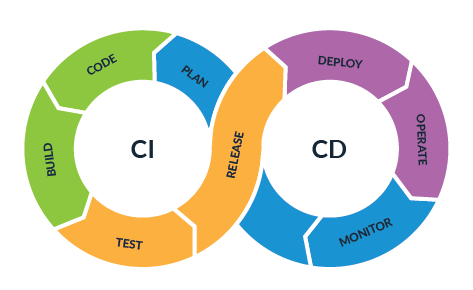
\includegraphics[scale=0.6]{../img/memoria/4_cicd.png}
	\label{img:4_cicd}
\end{figure}


CI (integración continua) es la práctica que permite integrar repetidas veces en pequeños segmentos temporales cambios en un repositorio de código. En este proyecto, para garantizar que los nuevos cambios introducidos en el repositorio son seguros y el \textit{merge} de las nuevas ramas no va a perjudicar versiones anteriores de código, se han automatizado distintos procesos (ejecución automática de \textit{tests}, análisis de código, escáneres de filtraciones de credenciales, etc.) utilizando las herramientas descritas en la sección~\ref{sec:herramientas_control_calidad}. Por otro lado, la entrega continua automatiza el despliegue de código a los usuarios finales, liberando a los equipos de operaciones de procesos manuales~\cite{cdciRedHat}. 

DevOps, sin embargo, abarca más. Esta cultura busca cubrir el ciclo completo del desarrollo de \textit{software}, desde la estructura del equipo hasta el control de versiones, y se sirve de las prácticas de CI/CD para lograr este fin.

\subsection{Gitflow}

Gitflow es un modelo alternativo de creación de ramas. Se caracteriza por contar con ramas de función y ramas principales, siendo recomendable aplicarlo en proyectos que trabajen con CD/CI~\cite{gitFlow}. En concreto, han sido utilizadas ramas principales y de desarrollo, fusionando el resultado de ésta última al final de cada \textit{sprint}. Debido a que en el equipo trabaja un único desarrollador, se ha desestimado crear una rama por \textit{feature} lanzada. Para garantizar que los \textit{merge} a la rama principal son seguros, se ha automatizado el uso de las herramientas desarrolladas en la sección~\ref{sec:herramientas_control_calidad}, generando \textit{builds} cada vez que se integra una rama nueva.

\subsection{Scrum}

Scrum es una metodología ágil basada en cuatro valores~\cite{scrumMaster2022}. Sintetizando sus principios, se puede deducir que se pretende valorar a los individuos por encima de las herramientas, el software apropiado a la documentación exhaustiva, la colaboración con el cliente y la habilidad de dar respuesta al cambio ante imprevistos.

Se describe en profundidad este método y cómo se ha desarrollado el trabajo siguiendo sus principios en los anexos.

\section{Herramientas}

Se muestra a continuación algunas de las herramientas más relevantes en el desarrollo del proyecto.

\subsection{Librerías}

Principalmente de Python, se destacan las siguientes utilidades:
\subsubsection{Scikit-Learn}

Una de las librerías referentes en el ámbito de \textit{machine learning} y Python. Además de utilizar la vertiente relacionada con aprendizaje automático, también se aprovecharon otras ramas del módulo como la de extracción de características de texto (TF-IDF)~\cite{sslearnRepo}. Debido a que proporciona una interfaz estándar para los clasificadores base de muchos algoritmos, posee muy buena documentación y es compatible con otras librerías, ha sido muy utilizada.

\subsubsection{sslearn}

Librería desarrollada por José Luis Garrido-Labrador dedicada al aprendizaje semisupervisado en Python. Utilizada para realizar comparaciones con algunos de los algoritmos implementados~\cite{sslearnRepo}.

\subsubsection{LAMDA}

\textit{Toolkit} escrito en Python con algunas implementaciones de los algoritmos más relevantes de aprendizaje semisupervisado~\cite{lamdasslRepo}. Nuevamente, ha sido utilizada como referente a la hora de realizar comparaciones contra las implementaciones propias~\cite{lamdasslPaper}.

\subsubsection{Beautiful soup}

Biblioteca de Python utilizada para extraer datos de ficheros \texttt{HTML} obtenidos mediante la realización de \textit{web scraping} a la hora de sintetizar vectores de características para la detección de \textit{phishing}. Se ha recurrido a ella, principalmente, cuando la obtención de ciertos campos en las etiquetas puede ser vulnerada mediante el uso de expresiones regulares corrientes~\cite{bs4Docs}.

\subsubsection{TLD}

Librería de Python utilizada para extraer dominios de alto nivel (TLDs) de los enlaces facilitados~\cite{tldLibreria}. Para evitar dependencias de biblitecas externas, en un primer momento se consideró trabajar con una lista del \textit{top} dominios más comunes (extraída de~\cite{tldLista}). Sin embargo, se descartó la idea debido a que no existe una forma intrínseca de saber qué cadenas son TLD y cuales son subdominios. Por ejemplo, \texttt{zap.co.it} es un subdominio ya que existe el TLD \texttt{co.it}. Sin embargo, en un país que no venda dominios de la forma \texttt{co.<<pais>>} sería un TLD~\cite{tldNogenerico}.

\subsubsection{NLTK}

\textit{Toolkit} de Python utilizado para trabajar con lenguaje natural. Su principal utilidad ha sido procesar palabras como \textit{tokens} para poder facilitar la implementación de algoritmos más complejos como TD-IDF o para analizar y procesar texto~\cite{nltk}.

\subsubsection{Otros}

Otras de las dependencias (estándar) del proyecto se enumeran a continuación.

\begin{itemize}
	\item \textbf{Requests}: permite realizar peticiones a distintas URLs, además de especificar parámetros relevantes en las mismas (como \textit{headers}, \textit{cookies}, \textit{proxies} o \textit{timeouts}).
	\item \textbf{urllib}: procesa URLs y las divide en campos.
	\item \textbf{re}: utilizada para aplicar expresiones regulares en Python.
	\item \textbf{Numpy, Pandas, Matplotlib}: utilizadas para tratar vectores, operaciones en \textit{arrays}, \textit{dataframes} y representar resultados.
\end{itemize}


\subsection{Extensiones y portales}

Principalmente utilizados para control de versiones y seguimiento de la metodología Scrum, se encuentran:

\subsubsection{ZenHub}

Zenhub es una extensión dedicada a la gestión de proyectos \textit{software} que se integra directamente con Github. Permite visualizar proyectos, \textit{sprints}, gráficos propios de Scrum y crear tableros. Debido a que el equipo de desarrollo cuenta con un único integrante, se considera la alternativa óptima (por ejemplo, a Jira) por su sencillez~\cite{zenhubHome}.

\subsubsection{Github}

Portal que permite alojar distintos repositorios en la nube~\cite{githubHome}. Ha sido escogido por ser una de las plataformas más populares, además de por permitir la interacción entre distintos usuarios. La gestión del \textit{backlog} del producto ha sido simulada mediante la creación de \textit{issues}.


\subsection{Programas}

En versión de escritorio, únicamente ha sido necesario recurrir a:

\subsubsection{KEEL}

Herramienta desarrollada en Java por distintas universidades españolas y financiada por el Ministerio de Educación y Ciencia~\cite{keelRepo}. Proporciona implementaciones de \textit{machine learning}, y ha sido utilizada para probar aquellos algoritmos no disponibles en las librerías de Python mencionadas anteriormente.

\subsubsection{\TeX{}Studio}
Editor de \LaTeX{} utilizado.

\subsubsection{Git BASH}
Emulador de BASH para Microsoft Windows que proporciona una terminal de línea de comandos de Git.

\subsection{Entorno de programación}

Relativo a la creación de un entorno que pueda ser reproducible, se facilita la siguiente información:

\begin{itemize}
	\item \textbf{Python}: lenguaje de programación interpretado de propósito general. Ha sido escogido para realizar este proyecto debido a la gran cantidad de paquetes dedicados a la ciencia de datos que posee~\cite{python}.
	\item \textbf{Visual Studio Code}: editor y depurador de código empleado junto a algunas de sus principales extensiones.
	\item \textbf{Entornos virtuales}: un entorno virtual es un directorio que contiene una instalación concreta de Python y los paquetes que se hayan decidido instalar~\cite{venvs}. Como se puede deducir, la correcta utilización de los entornos virtuales conlleva muchas ventajas, como tener varios paquetes sin conflictos entre ellos o evitar corromper la instalación base si se está probando algún elemento nuevo.
	\item \textbf{Conda}: es un sistema de gestión de paquetes y entornos \textit{opensource}. Es especialmente útil a la hora de realizar trabajos de ML ya que posee librerías como SciPy y TensorFlow~\cite{conda}.
\end{itemize}

\subsection{Control de calidad}
\label{sec:herramientas_control_calidad}

Siguiendo los principios de CD/CI, se ha procurado garantizar la calidad del código desarrollado. Para ello se han utilizado diversas herramientas, entre ellas:

\begin{itemize}
	\item \textbf{SonarCloud}: se trata de un servicio de análisis estático de código que notifica diversos parámetros a revisar como \textit{codesmells}, \textit{bugs} o vulnerabilidades. Se ha integrado en el repositorio con la intención de realizar código limpio y aumentar la calidad del proyecto~\cite{sonarCloud}.
	\item \textbf{DeepSource}: se trata de una plataforma que fusiona el análisis estático de código, SAST (\textit{static application security testing}), cobertura de código y más para mejorar la calidad de los proyectos. Además, posee un \textit{bot} que realiza ciertas correcciones automáticas (por ejemplo, modifica errores de documentación) y facilita \textit{badges} para los repositorios~\cite{deepSourceBot}.
	\item \textbf{Travis CI}: se ha utilizado el servicio para la realización automática de \textit{tests} cada vez que se actualiza el repositorio. Para ello, se ha configurado una \textit{build} y recreado el entorno del programador. De este modo, antes de realizar un \textit{merge} a la rama principal se puede comprobar rápidamente si las pruebas siguen pasando, lo que mejora la integración y despliegue continuo~\cite{travisCI}.
	\item \textbf{Git Guardian}: herramienta que escanea los repositorios en busca de posibles filtraciones de credenciales, se ha utilizado para garantizar que las contraseñas de acceso a bases de datos y otros secretos permanezcan ocultos. Ha sido incluida, junto con las anteriores, en el flujo de Git~\cite{gitGuardian}.
\end{itemize}


\subsection{\textit{Scripts}} 

En algunos casos no se han encontrado soluciones de terceros y ha sido necesario implementar \textit{scripts} propios. Los mas relevantes se citan a continuación:

\subsubsection{\textit{Script} para levantar proxies SOCKS5}
\label{sec:script_tor}
Durante la extracción de vectores de características, se realizan peticiones a páginas de \textit{phishing}. Para garantizar que estas páginas no puedan rastrear desde donde se ha realizado la petición, se han utilizado \textit{proxies} que implementan el protocolo SOCKS5.

Para ello, se ha implementado en python un \textit{script} auxiliar que levanta en paralelo tantas instancias de Tor como se soliciten, y mantiene los hilos vivos hasta que se interrumpa la ejecución del \textit{script}.

Por cada instancia de Tor que se quiera levantar, se necesita un fichero \texttt{torrc} en el directorio \texttt{/etc/tor/}~\cite{TorFicherosTor}. Cada una de ellas debe tener, además, su propio puerto de control, su propio puerto \textit{socks} y su directorio de datos. Por ello, se ha creado una clase auxiliar que genera estos ficheros. Para levantar la instancia simplemente ha de ejecutarse el comando \texttt{tor -f /etc/tor/torrc.x} (siendo $x$ el número de la instacia correspondiente), aunque se ha decidido, además, dirigir la salida al fichero \texttt{/dev/null}. Es importante destacar que el puerto de control debe ser el siguiente al puerto \textit{socks}. Teniendo en cuenta que los puertos por defecto de Tor son el 9050 y el 9051, se puede incrementar partiendo de esos números\footnote{Solución basada en la respuesta del usuario <<zkilnbqi>> en Stack Overflow \url{https://stackoverflow.com/questions/14321214/how-to-run-multiple-tor-processes-at-once-with-different-exit-ips}.}. Para comprobar que la instancia levantada funciona correctamente, se hace una petición a \url{http://ipinfo.io/ip} y se comprueba con una expresión regular que la dirección obtenida es la correcta. De este modo, se sabe que el \textit{proxy} HTTP levantado funciona, y se puede utilizar redireccionando las peticiones oportunas a través del \textit{proxy} \texttt{socks5h://127.0.0.1:$y$} (donde $y$ es el puerto \textit{socks} de la instancia correspondiente). Para que pueda ser usado en código, se ha generado un \texttt{JSON} donde se incluyen como diccionarios los \textit{proxies} disponibles, y se utilizan en combinación con la librería Requests.

Debido a que el puerto Tor queda <<a la escucha>> en la máquina local (está esperando que se realice una conexión), no conlleva ningún riesgo. Para cerrar el puerto, es suficiente con parar el proceso que esté ejecutando el \textit{script}. Se puede comprobar ejecutando en una terminal el comando \texttt{sudo lsof -i:$y$} (nuevamente, $y$ es el puerto \textit{socks} levantado). Cuando el \textit{script} esté funcionando, la salida del comando mostrará diversos campos, como el propio comando (Tor), el PID, el nombre (\textit{listen}). Si el \textit{script} se para, el comando no mostrará salida, lo que implica que el puerto no está abierto~\cite{checkOpenTorPorts}.
\capitulo{5}{Aspectos relevantes del desarrollo del proyecto}



\section{Experimentación}

\subsection{Algoritmos de aprendizaje semisupervisado}

\subsubsection{\textit{Co-Forest}}

Para evaluar la calidad del método, se han realizado distintos experimentos con los \textit{dataset} incluídos en la librería \textit{SKlearn} dedicados a la clasificación. Estos son los mostrados en la tabla~\ref{tabla_datasets_sklearn}. El parámetro $n$ representa el número de instancias que contiene un determinado conjunto de datos, mientras que el parámetro $m$ muestra el número de atributos que contiene cada una de esas instancias.

\begin{table}
	\small
	\begin{centering}
		
		\begin{tabular}{@{}p{4em} p{20em} r r r @{}}
			\toprule
			\textbf{Nombre} & \textbf{Descripción} & \textbf{Clases} & $n$ & $m$\\ 
			\midrule
			
			Iris & Conjunto de instancias pertenecientes a diferentes tipos de plantas de la especie Iris. & 3 & 150 & 4 \\\\
			Dígitos & Conjunto de instancias que representan una imagen de 8x8 perteneciente a un dígito. & 10 & 1797 & 64 \\\\
			Vino & Conjunto de instancias pertenecientes tres clases de vino con sus parámetros estimados mediante análisis químico & 3 & 178 & 13 \\\\
			Cáncer de Mama & Conjunto de instancias que representan parámetros de distintas mujeres que pueden padecer o no cáncer (clasificación binaria). & 2 & 569 & 30 \\
		\end{tabular}
		
	\end{centering}
	\caption{Descripción de los \textit{datasets} utilizados para probar el \textit{co-forest}.}
	\label{tabla_datasets_sklearn}	
\end{table}


Se han realizado diferentes experimentos: algunos relacionados con la fase de entrenamiento y otros con el algoritmo una vez finalizado.

\paragraph{Fase de entrenamiento}

Como se ha desarrollado en los conceptos teóricos, la fase de entrenamiento en el \textit{co-forest} es iterativa, y finaliza cuando ningún árbol recibe nuevas pseudo-etiquetas que puedan cambiar su comportamiento (en la fase de re-entrenamiento).

Se ha querido estudiar la evolución de la precisión del algoritmo durante la fase de entrenamiento para los cuatro conjuntos de datos definidos en la tabla~\ref{tabla_datasets_sklearn}. Para ello, se ha realizado una gráfica comprobando cómo evoluciona la precisión del algoritmo en función de la iteración en la que se encuentre.

Para garantizar que los resultados obtenidos no son producto de una partición concreta de los datos, se ha realizado validación cruzada (con 10 particiones). Por lo tanto, el porcentaje de datos utilizados para el entrenamiento es el $90\%$ del total. Los datos de entrenamiento, a su vez, se dividen en etiquetados y no etiquetados. En este caso, el 20\% representa los datos etiquetados, y el 80\% los no etiquetados, como se puede observar en la imagen~\ref{5_entrenamiento_particiones}. Se han utilizado 20 árboles.

\begin{figure}[h]
	\caption{Gráfica que representa la distribución de los datos.}
	\centering
	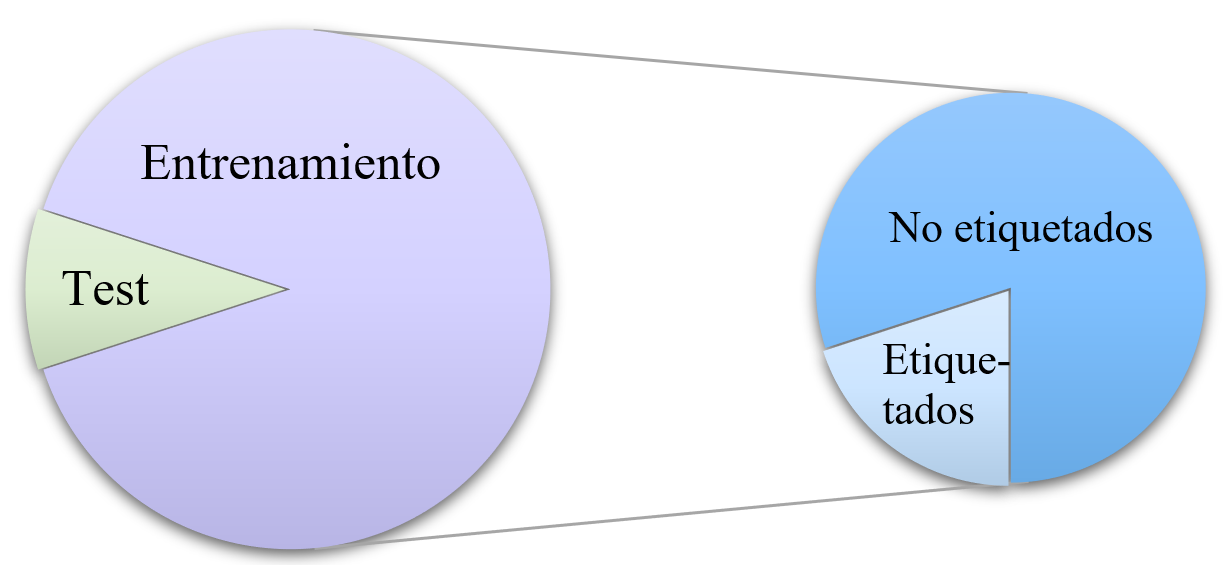
\includegraphics[width=\textwidth]{../img/memoria/5_entrenamiento_particiones}
	\label{5_entrenamiento_particiones}
\end{figure}


 La precisión media obtenida se puede ver representada en la gráfica~\ref{5_coforest_precision-iteraciones}. Es destacable que, dependiendo de los datos que se utilicen para entrenar el \textit{co-forest}, puede variar el número de iteraciones que se necesiten (incluso dentro de un mismo \textit{dataset}). Por ello, siempre se representa el número máximo de iteraciones realizadas, y para no deformar la media, se ha considerado que el valor de las iteraciones inexistentes es el mismo que el valor obtenido en la última iteración (ya que si, el algoritmo siguiese, el resultado devuelto sería igual debido a que no se re-entrenaría ningún árbol).

\begin{figure}[h]
	\caption{Gráfica que representa la precisión del modelo en función de la iteración en la que se encuentre.}
	\centering
	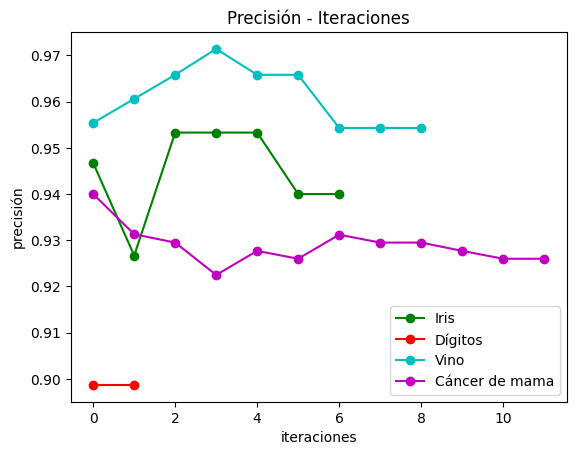
\includegraphics[width=\textwidth]{../img/memoria/5_coforest_precision-iteraciones}
	\label{5_coforest_precision-iteraciones}
\end{figure}


Como se puede comprobar, en general los resultados obtenidos no son satisfactorios debido a que la precisión alcanzada en la última iteración es inferior a la obtenida en la iteración $0$ (cuando todavía no se ha realizado entrenamiento semi-supervisado y se cuenta con un \textit{random forest} normal). Sin embargo, sí se puede observar como en general, en las iteraciones centrales, la precisión inicial es mejorada.

Si se observa con más detenimiento cada conjunto de datos individualmente (gráfica~\ref{5_coforest_precision-iteraciones_individual}), se puede observar que la desviación típica varía considerablemente, por lo que se puede deducir que el modelo podría llegar a ser utilizable si el conjunto de entrenamiento es el adecuado.

\begin{figure}[h]
	\caption{Gráfica que representa, para cada conjunto de datos, la precisión media del modelo en función de la iteración en la que se encuentre junto con la desviación típica para 10 experimentos.}
	\centering
	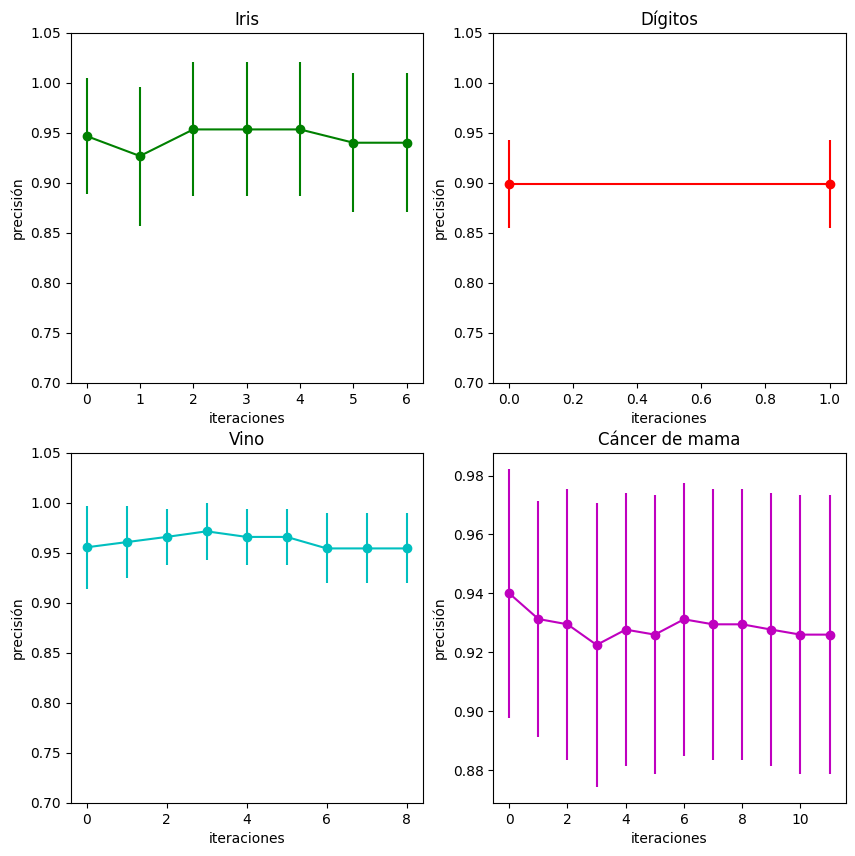
\includegraphics[width=\textwidth]{../img/memoria/5_coforest_precision-iteraciones_individual}
	\label{5_coforest_precision-iteraciones_individual}
\end{figure}


Además, también se ha querido evaluar cómo varía el tiempo de entrenamiento en función del número de instancias utilizadas. Para ello, se ha trabajado con el \textit{dataset} que contiene un mayor número de datos, y los resultados obtenidos se pueden observar en la gráfica~\ref{5_coforest_tiempo-instancias}. Como se puede observar, sigue un crecimiento aproximadamente lineal. La velocidad, en este caso, es alta, pero cabe recordar que depende en gran medida del número de árboles utilizados y de las iteraciones que estos realicen (en este caso, 2).

\begin{figure}[h]
	\caption{Gráfica que representa la evolución del tiempo de entrenamiento en función del número de instancias utilizadas.}
	\centering
	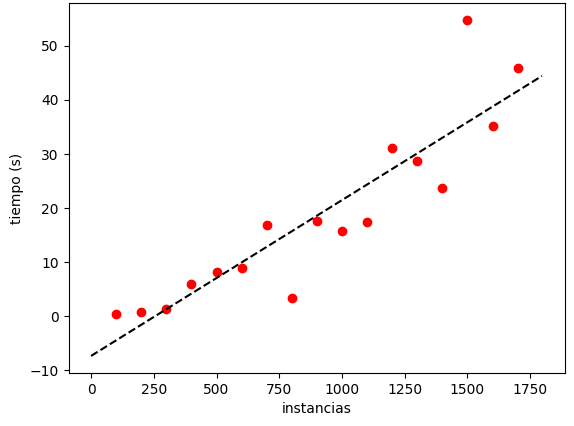
\includegraphics[width=\textwidth]{../img/memoria/5_coforest_tiempo-instancias}
	\label{5_coforest_tiempo-instancias}
\end{figure}
\par


\paragraph{Comportamiento general}

En este apartado de la experimentación, se ha querido evaluar cómo se comporta el \textit{co-forest} en función del porcentaje de datos que se utilice para el entrenamiento. Nuevamente, se han utilizado 20 árboles, y la división del conjunto de datos de entrenamiento se ha mantenido: 20\% etiquetados y 80\% no etiquetados.

Como se puede comprobar en la gráfica~\ref{5_precision-porcentaje_entrenamiento}, se sigue el comportamiento esperado, y por lo general a más instancias utilizadas para entrenar el modelo, mejor comportamiento desarrolla. Nuevamente, recalcar que el resultado obtenido es la media de 10 experimentos realizados.

\begin{figure}[h]
	\caption{Gráfica que representa la precisión media del modelo en función del porcentaje de datos utilizados para el entrenamiento.}
	\centering
	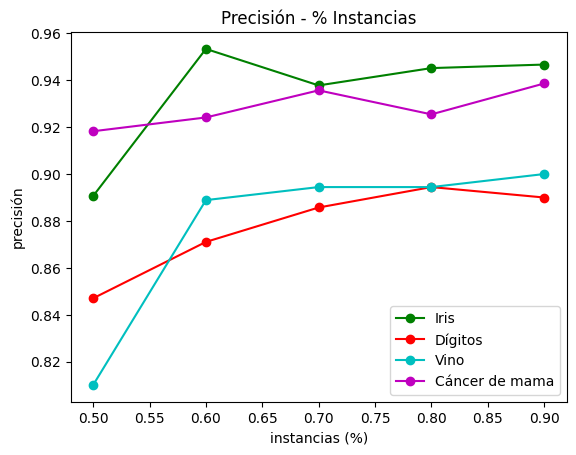
\includegraphics[width=\textwidth]{../img/memoria/5_precision-porcentaje_entrenamiento}
	\label{5_precision-porcentaje_entrenamiento}
\end{figure}
\par

Se representa además, en la gráfica~\ref{5_precision-porcentaje_entrenamiento_individual} la desviación media obtenida en los 10 experimentos para cada conjunto de datos.

\begin{figure}[h]
	\caption{Gráfica que representa, para cada conjunto de datos, la precisión media del modelo y su desviación en función del porcentaje del conjunto utilizado para el entrenamiento.}
	\centering
	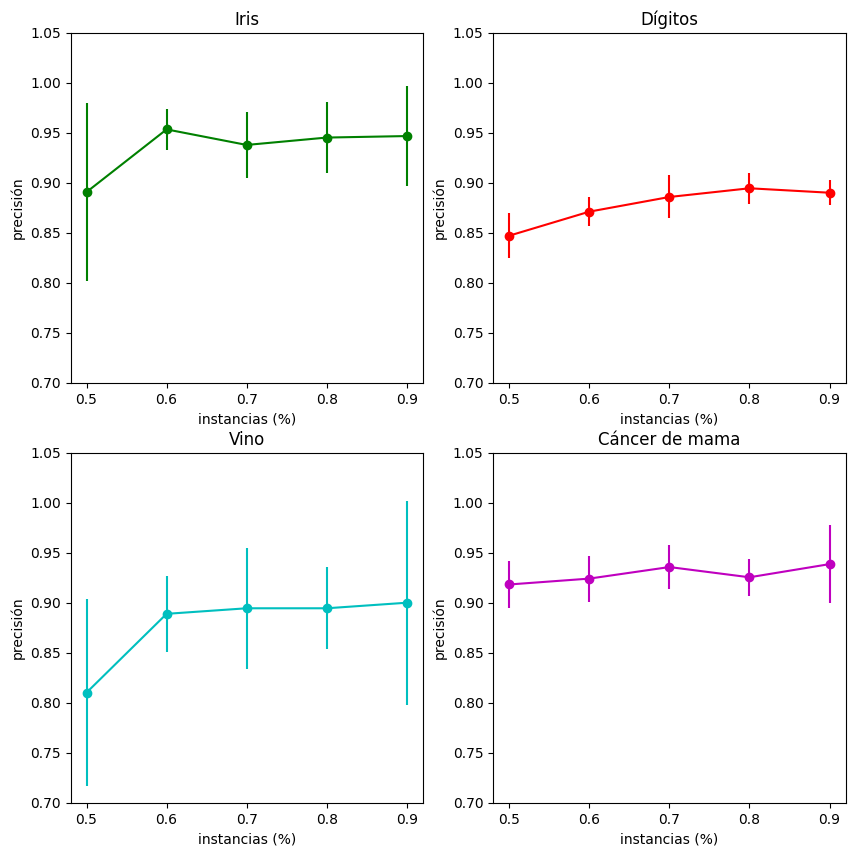
\includegraphics[width=\textwidth]{../img/memoria/5_precision-porcentaje_entrenamiento_individual}
	\label{5_precision-porcentaje_entrenamiento_individual}
\end{figure}
\par

\capitulo{6}{Trabajos relacionados}

Dentro de este proyecto se pueden diferenciar tres líneas de investigación:


\section{Aprendizaje semisupervisado}

Como principal referente, se ha utilizado el artículo de Jesper E. van Engelen y Holger H. Hoos \citep{engelen-hoos}. En él, se expone una clasificación general de los principales tipos de métodos derivados del aprendizaje semisupervisado y sus características. Auxiliarmente, también ha sido consultado el documento de Triguero, García y Herrera \citep{triguero-garcia-herrera}. 


\section{Aprendizaje semisupervisado aplicado a la detección de ataques en sistemas de recomendación}

En este caso, el artículo fundamental es \citep{zhou-duan}. En este documento, se propone un método de detección basado en Co-Forest y se producen distintas comparativas con otros algoritmos para comprobar su eficacia, consiguiendo unos resultados muy aceptables. También es muy relevante citar el trabajo de \citep{zhiang-junjie}, puesto que propone una aproximación Naive Bayes para separar perfiles de atacantes de perfiles genuinos y además propone los datasets que son utilizados posteriormente por Zhou y Duan (Amazon, Netflix y MovieLens).

\section{Ataques en sistemas de recomendación}

La importancia de proteger los sistemas de recomendación ha sido contemplada desde principio de siglo, siendo común la proposición de otros tipos de aprendizaje para detectar los ataques.

Respecto a la descripción de los tipos de intrusión, la correcta definición formal (matemática) de sus parámetros y una recopilación de la gran mayoría de ataques existentes, es fundamental referenciar el artículo de \citep{mingdan-qingshan}. Previo a este documento,también es relevante contemplar otros trabajos, como la conferencia de \citep{lam-riedl}, donde se propone utilizar como datasets los conjuntos de películas o el paper de \citep{mahony}, que define los modelos de construcciones en base a conocimiento del sistema y pone a prueba la robustez de los recomendadores evaluando su estabilidad y precisión ante la presencia de perfiles inyectados (análisis matemático muy completo).
\capitulo{7}{Conclusiones y Líneas de trabajo futuras}

En este último capítulo de la memoria se pretende enumerar algunos de los aprendizajes extraídos durante la realización del proyecto, además de proponer ideas de mejora para refinar el desempeño de la propuesta presentada.

Es destacable que los puntos desarrollados a continuación son de carácter general. Si se quieren leer conclusiones concretas acerca de algoritmos o aproximaciones de detección relacionadas con la ciberseguridad, se recomienda consultar el capítulo~\hyperref[s:5]{5} de la memoria.

\section{Conclusiones}

Debido a que se han extraído aprendizajes de diversa índole durante el desarrollo del proyecto, se ha decidido clasificarlos en tres secciones distintas. En un primer lugar, se van a exponer conclusiones <<científicas>> (referentes a la experimentación). Posteriormente, conclusiones <<técnicas>> (asociadas con el desarrollo del producto \textit{software}). Por último, se enumeran algunas conclusiones <<personales>> (relacionadas con el aprendizaje propio de la desarrolladora durante el proyecto).

\subsection{Científicas}

Con respecto a las metodologías de modelado y solución de problemas mediante aprendizaje automático, se destaca la importancia de <<no dejarse llevar>> por los algoritmos y prestar verdadera \textbf{atención a los métodos de extracción y preparado de datos}. Es infinitamente más complicado (y, por lo tanto, consume más recursos) extraer un \textit{dataset} apropiado que encontrar algoritmos de clasificación adecuados para las tareas de clasificación.

Del método de detección de \textit{phishing} se destaca la \textbf{dificultad de realizar correctamente \textit{web scraping}}. Es indudable la gran variedad de formas que existen en la programación \textit{web} para conseguir un mismo objetivo, y lograr una aproximación <<universal>> es, por lo tanto, un objetivo muy ambicioso.

Destacable además la importancia de \textbf{parametrizar correctamente los algoritmos}. Se ha comprobado mediante la experimentación con el \textit{co-forest}, como pequeños cambios pueden suponer un impacto en el desempeño de un modelo, por lo que es fundamental que los ajustes sean corectos.

Sin embargo, la conclusión más significativa extraída en esta sección es que \textbf{no siempre se obtienen resultados brillantes, y eso está bien}. Es igual de importante descubrir una aproximación nueva que cerrar líneas de investigación que tal vez no sean tan relevantes (aunque lamentablemente esto no suele ser fácilmente publicable en revistas científicas).

\subsection{Técnicas}

Indudablemente se ha de mencionar la importancia de introducir \textbf{herramientas de control de calidad en los repositorios} desde el momento de su creación. En este proyecto se introdujo el concepto de calidad cuando ya estaba avanzado, lo que conllevó enfrentarse a un gran número de defectos que podrían haber sido evitados poco a poco durante fases tempranas del desarrollo. También es fundamental mencionar la necesidad de \textbf{evaluar} las salidas (o reportes) que nos proporcionan estas herramientas y saber analizar falsos positivos o no actuar en situaciones de <<peligro>> (si, por ejemplo, no se dispone de una \textbf{batería robusta de pruebas} que verifique la posible introducción de defectos de regresión).

Por otro lado, y respecto a la programación \textit{web}, se ha aprendido la importancia (y dificultad) de realizar un \textbf{despliegue correcto}. El lanzamiento del producto desarrollado ha supuesto más de un reto y, muchas, veces, sin solución <<gratuita>>. Sin embargo, es destacable que siempre se pueden encontrar alternativas (en este proyecto, por ejemplo, la solución a los \textit{timeouts} en Heroku se ha logrado mediante contenedores de Docker que pueden ser probados en una instalación local). También es reseñable la correcta configuración de los servidores de despliegue, ya que pueden surgir problemas (por ejemplo, de concurrencia), que no se encontraban en los servidores de desarrollo.

Es destacable, además, la relevancia de (cuando sea posible) \textbf{depender del menor número de herramientas de terceros}, ya que pueden generar conflictos entre ellas o incluso introducir fallos de seguridad.

Por útimo, mencionar la gran importancia de contar con una correcta \textbf{documentación}, aunque suponga desviar una gran cantidad de recursos de desarrollo (sobre todo, a nivel temporal).

\subsection{Personales}

En un primer lugar, se destaca la \textbf{importancia de poseer un juicio crítico} con el trabajo propio y ajeno, y saber evaluar en condiciones justas el conocimiento extraído. Se ha podido comprobar como ciertos \textit{papers} publicados plantean aproximaciones como <<universales>>, cuando en realidad funcionan por ajustarse a un conjunto de datos en concreto y suponer generalizaciones que no se mencionan.

Relacionado con lo anterior, también se destaca la capacidad de saber \textbf{analizar el contenido de las publicaciones científicas} y no suponer que todo lo expuesto en ellas es indudablemente correcto. Se ha verificado como, en muchos \textit{papers}, hay detalles de implementación que no se enumeran de forma explícita y es el desarrollador quien debe tomar decisiones.

Conviene no pasar por alto tampoco el \textbf{estudio de literatura previo a la selección de una línea de investigación}, ya que muchas veces resulta <<invisible>> y es un trabajo considerable a realizar. Por ejemplo, en este trabajo, antes de decidir investigar los ataques a sistemas de recomendación y \textit{phishing}, se realizó una investigación en la literatura de la materia leyendo y comparando diversos tópicos como intrusión en redes, localización de \textit{markets} ilegales en la \textit{deep web}, detección de \textit{malware} o descubrimiento de dispositivos anómalos en redes IoT.

Por otro lado, se destaca cada vez más la \textbf{importancia de saber adaptarse antes que dominar a la perfección todo tipo de tecnologías}. En muchas ocasiones, se ha tenido que aprender nuevas herramientas o paradigmas de programación que no se conocían, y no siempre se dispone del tiempo necesario para <<convertirse en un experto>> de una tecnología nueva. Por ello, es fudamental acostumbrarse a buscar lo que se necesite y saber aplicarlo.

Por último, subrayar la importancia de la \textbf{constancia frente a la motivación}. En un trabajo de estas características (donde una única una persona es la encargada de investigar, probar, desarrollar, documentar e implementar), es fundamental tener la disciplina necesaria para trabajar a diario, aunque haya días que supongan un esfuerzo \textit{extra} o se tenga más trabajo externo que hacer.


\section{Líneas de trabajo futuras}

El mundo de la ciberseguridad se encuentra en constante cambio, y los distintos tipos de ataques existentes avanzan con el fin de ser indetectables. Por ello, es fundamental anticiparse a dicha evolución y establecer líneas de trabajo que mejoren las aproximaciones actuales.

A continuación, se van a detallar algunos aspectos que se podrían implementar para refinar el proyecto. Nuevamente, van a ser desglosados en distintas categorías:

\subsection{Algoritmos de aprendizaje semisupervisado}

Respecto al estudio e implementación de algoritmos de aprendizaje semisupervisado, se sugiere:

\begin{itemize}
	\item \textbf{Implementar nuevos algoritmos}: y validar los resultados obtenidos con el fin de aumentar la oferta de \textit{ensembles} en la \textit{web}.
	\item \textbf{Mejorar las implementaciones actuales}: introduciendo, por ejemplo, computación paralela.
\end{itemize}

\subsection{Detección de \textit{phishing}}

Relacionado con la detección y clasificación de páginas fraudulentas o legítimas, se propone:

\begin{itemize}
	\item \textbf{Investigar nuevos métodos de extracción de vectores de características}: con el fin de mejorar la detección de \textit{phishing}\footnote{Algunas ideas ya se encuentran registradas y se pueden consultar en el \textit{issue} \#132 del repositorio \url{https://github.com/phf1001/semisupervised-learning-in-cibersecurity/issues/132}}.
\end{itemize}


\subsection{Krini (página \textit{web})}

Relativo al producto \textit{software} entregado, se plantea:

\begin{itemize}
	\item \textbf{Nuevos algoritmos}: incorporar nuevos algoritmos de aprendizaje para aumentar la diversidad de modelos existentes.
	\item  \textbf{Mayor variedad de estimadores base}: incluir nuevos estimadores base de la API de Scikit-Learn y ofrecer una mayor flexibilidad a la hora de configurar estos clasificadores.
	\item \textbf{Nuevos métodos de detección}: basados en la extracción de vectores de características alternativos (se podría, incluso, analizar las URLs utilizando varios procedimientos).
	\item \textbf{Internacionalizar}: atendiendo a las características de las culturas objetivo y adaptando no solo el idioma (también iconos, colores, etc.).
	\item \textbf{Gestión de usuarios}: incluir un nuevo caso de uso que permita a los administradores gestionar usuarios desde la aplicación.
	\item \textbf{Despliegue}: buscar alternativas a Heroku (que soporten peticiones superiores a 30 segundos) con el fin de facilitar el acceso completo a la aplicación.
\end{itemize}


\bibliographystyle{plain}
\bibliography{bibliografia}

\end{document}
